\chapter{VBF Higgs Measurement in the \wwlnln~Decay Mode}
\label{chap:analysis}

%The \hwwlnln analysis is split into three jet bins \Njet$=$~0,1, and 2
%or more. This thesis focuses on the measurement of the VBF rate in the
%\Njet$\geq{2}$ bin. Unless otherwise noted, the gluon fusion \hww
%process is treated as a background. 

\section{Overview}
%
The primary aim of this analysis is to measure the rate at which the
Higgs boson is produced via vector boson fusion. Previous Higgs
measurements, including the ones in which the Higgs was discovered,
have lumped together ggF, VBF, and VH into a single signal controlled
by the the same strength. This analysis, by contrast, considers only the
Higgs processes with two $VVH$ couplings, VBF and $VH$, to be
signal, with the assumption that SM ggF production at
$m_H=125$~\gev~has already been discovered. Therefore, the
optimization of the analysis was done at $m_H=125$~\gev~, with ggF $H$
being produced at the SM rate included in the background-only hypothesis. In
addition to measuring the rate of VBF production, the probability of
observing the data assuming the null hypothesis to be true is
extracted. In the presence of an excess in the observed data with
respect to the background-only hypothesis, this
corresponds to the statistical significance of the excess.

Dedicated VBF rate measurements have been done in ATLAS in the \wwlnln
channel with 25~fb$^{-1}$ of data, with an observed significance of 2.5$\sigma$ and
a measured signal strength of $1.66\pm 0.79$ times the
$\sigma_{\mathrm{VBF}}\cdot{\mathrm{Br}}$ predicted by the
SM~\cite{bib:hww_moriond_2013}. The analysis presented in this thesis
improves on the previous analysis in
many respects, most notably the use of a multivariate technique called
a boosted decision tree (BDT) which is explained in chapter
XX. This chapter details the BDT-based VBF analysis, describing in
detail the selection of physics objects and events
(sections~\ref{chap:analysis:sec:objects} and~\ref{chap:analysis:sec:event_selection}), the
BDT inputs and and validation
(sections~\ref{chap:analysis:sec:bdt_inputs} and~\ref{chap:analysis:sec:bdt_validation}),
data-driven background estimation
methods (section~\ref{chap:analysis:sec:dd_backgrounds}), systematic
uncertainties (section~\ref{chap:analysis:sec:systematics}),
and finally the results (section~\ref{chap:analysis:sec:results}). A
more in depth discussion of the statistical methods and results can be
found in the following chapter. This chapter will conclude with a
summary of the analysis of a smaller dataset collected at $\sqrts =
7 \tev$ in 2011, as well as a brief description of the \hww analyses
in other jet bins


\section{Data and MC samples}
\label{chap:analysis:sec:data_mc}
%
The analysis is performed on $pp$ collision data recorded by the ATLAS
detector, discussed in detail in section XX. Data are partitioned in
time into runs and if the detector subsytems are functioning
sufficiently well in for a given run (should I go into more detail?),
the data for that run are included. This thesis focuses on
20.3~fb$^{-1}$ of data collected in 2012 at \sqrts$=8$~\tev. For the
final statistical results, a smaller dataset of
4.5~fb$^{-1}$ at \sqrts$=7$~\tev is included. This analysis is briefly
discussed in section XX. 

Monte Carlo simulations are relied on for the prediction of signal and
background observables. The hard scattering process, subsequent
showering and hadronization of final state quarks and gluons, and the
response of the detector are all simulated with MC programs. The
absolute predictions are then obtained by scaling the MC distributions
by the factor $\frac{\mathcal{L}\cdot{\sigma}}{N_{\mathrm{total}}}$,
where $\mathcal{L}$ is the integrated luminosity, $\sigma$ is the best
available cross section calculation for the process, and
$N_{\mathrm{total}}$ is the total number of events generated, or in
the case of weighted MC, the sum of
weights. Table~\ref{chap:analysis:tab:mc_summary} summarizes the MC
programs used for each signal and background process, as well as the
cross section to which the prediction is scaled. Each cross section
includes the relevant branching fraction for the $\ell\nu\ell\nu$
final state integrated over all lepton combinations. 

\begin{table}[h]
  \centering
%{\small
\resizebox{0.8\textwidth}{!}{
  \begin{tabular}{llrr}
    \hline
    Process & Generator & \hspace*{-3mm}$\sigma\cdot\mathrm{Br}$(8TeV)
  (pb) \\%\hspace*{-3mm}$\sigma\cdot\mathrm{Br}$(7TeV) (pb)\\
    \hline\hline
    VBF $H\rightarrow WW$  & \POWHEG~+~\PYTHIAns8 & $36\cdot 10^{-3}$ \\%& $28\cdot 10^{-3}$ \\
    ggF $H\rightarrow WW $  & \POWHEG~+~\PYTHIAns8 & 0.435\\% &  0.341 \\
    $WH/ZH$ $H\rightarrow WW $ & \PYTHIAns8 (\PYTHIAns6) & $25\cdot 10^{-3}$ \\% & $21\cdot 10^{-3}$ \\
    \hline
    $\ttbar$ dileptonic & \POWHEG~+\PYTHIAns6 & 26.6 \\%& 18.6\\
    % single top NB: sum s-ch, t-ch, Wt
    $tW/tb$ leptonic      & \POWHEG~+~\PYTHIAns6 & 4.17\\% & 3.15
    $tqb$ leptonic        & \textsc{AcerMC}~+~\PYTHIAns6 & 28.4\\% & 20.7\\         % checked
    QCD $WW + 2$ jets & \SHERPA & 0.568\\% & - \\
    EW $WW + 2$ jets & \SHERPA & 0.039\\% & 0.027\\
    $gg\rightarrow WW$ & \GGTOWW~+~\HERWIG & 0.20\\% & 0.14\\
    % W+jets NB: BR to single lepton flavour multiplied by 3 flavours
    inclusive $W$ & \ALPGEN~+~\HERWIG & $37\cdot 10^{3}$\\% & $31\cdot 10^{3}$\\
    % Z/gamma*+jets NB: BR to single lepton flavour multiplied by 3 flavours
    inclusive $Z/\gamma^{\star} (m_{ll} \ge 10 GeV)$ & \ALPGEN~+~\HERWIG & $16.5\cdot 10^{3}$\\% & $14.9\cdot 10^{3}$\\
    EW $Z/\gamma^{\star}$ & \SHERPA & 5.36 (inc. t-ch)\\% & 2.26\\
    $W(Z/\gamma^{\ast}) $     & \POWHEG~+~\PYTHIAns8 & 12.7\\% & 10.8\\
    $W(Z/\gamma^{\ast}) (m_{(Z/\gamma^{\ast})} < 7~\GeV)\ $ & \SHERPA & 12.2\\% & 10.6 \\ % checked
    $Z^{(\ast)}Z^{(\ast)} \to 4l(2l2\nu)$ & \POWHEG~+~\PYTHIAns8 & 0.73(0.50)\\% & 0.64(0.42)\\
    EW $WZ + 2$ jets  & \SHERPA & $13\cdot 10^{-3}$\\% & $8.5\cdot 10^{-3}$\\
    EW $ZZ + 2$ jets $(4l,ll\nu\nu)$ & \SHERPA & $73\cdot 10^{-5}(12\cdot 10^{-4})$\\% & $53\cdot 10^{-5}(8.8 \cdot 10^{-4})$\\
    $W\gamma$ & \ALPGEN~+~\HERWIG & 369\\% & 313\\
    $Z\gamma$($p_{T}^{\gamma} > 7GeV$) & \SHERPA & 163\\% & - \\
    \hline
  \end{tabular}
}
\caption[MC sample summary.]{MC sample summary with corresponding
cross sections.}
  \label{chap:analysis:tab:mc_summary}
\end{table}

The signal process, VBF Higgs production in the \ww decay channel, is
modeled with \POWHEG~\cite{bib:Nason:2009ai} interfaced to \PYTHIAns8~\cite{bib:Sjostrand:2007gs} for the parton
shower. The cross
section is computed at NLO in QCD and EW~\cite{Ciccolini:2007jr,Ciccolini:2007ec,Arnold:2008rz}, with approximate
NNLO QCD corrections~\cite{Bolzoni:2010xr}. The branching fraction for
the \ww decay for this VBF process and the other Higgs processes in
this analysis is derived from the \hdecay
program~\cite{Djouadi:1997yw}. The final $\sigma\cdot{\mathrm{Br}}$~is
0.036~pb at $m_H = 125$~\gev. Because $VH$ Higgs production probes the
same Higgs coupling as VBF, these processes are lumped into
signal. The cross sections for $ZH/WH$ are calculated at NNLO in
QCD~\cite{Han:1991ia,Brein:2003wg} with NLO EW radiative
corrections~\cite{Ciccolini:2003jy}. At $m_H = 125$~\gev the resulting
cross sections are $\sigma_{ZH} = 9.4$~fb and $\sigma_{ZH} = 15.9$~fb
for the processes in which the $W$ bosons from the Higgs decay
leptonically. 

The ggF$+2$j process is also simulated with \POWHEG~\cite{bib:Alioli:2008tz} interfaced with
\PYTHIAns8. The cross section is computed at NNLO in
QCD~\cite{Djouadi:1991tka,Dawson:1990zj,Spira:1995rr,Harlander:2002wh,Anastasiou:2002yz,Ravindran:2003um},
with NLO electroweak corrections~\cite{Aglietti:2004nj,Actis:2008ug}
and soft gluon resummations up to
next-to-next-to-leading-log (NNLL)~\cite{Catani:2003zt}. Due
to known deficiencies in the Higgs $p_T$ spectrum in \POWHEG, the
Higgs $p_{\mathrm{T}}$ is re-weighted to the NLO + NNLL prediction
from \HqT~\cite{deFlorian:2011xf}. The $\sigma\cdot{\mathrm{Br}}$ is
0.435~pb, a factor of 12 larger than VBF. 

Top background is comprised mainly of \ttbar, with smaller
contributions from $s$ and $t$ channel single top and $Wt$. The
hard scatter for \ttbar~is simulated in \POWHEG~\cite{bib:Frixione:2003ei} at NLO in QCD,
while \PYTHIAns6~\cite{bib:Sjostrand:2006za} is used for parton showering and
hadronization. The LO PDF set CTEQ6L1 is used with \PERUGIA~2011 as
the underlying event tune. For ST,
$s$ channel and $Wt$ use \POWHEGns~\cite{bib:Alioli:2009je,bib:Re:2010bp}~+~\PYTHIAns6 as well, while
\textsc{AcerMC}~\cite{bib:Kersevan:2004yg}~+~\PYTHIAns6 is used to model $t$-channel ST. The same
PDF and UE tune is used for all top processes. The
\ttbar~normalization is scaled to the cross section for $pp$
collisions at \sqrts~$=8$~\tev~for a top quark mass of
$172.5 \gev/c^2$, $\sigma_{t\bar{t}}=252.9^{+15.3}_{-16.3}$~pb. This
value has been calculated at NNLO in QCD including a resummation of
NNLL soft gluon
terms~\cite{bib:Cacciari:2011hy,bib:Beneke:2011mq,bib:Baernreuther:2012ws,bib:Czakon:2012zr,bib:Czakon:2012pz,bib:Czakon:2013goa,bib:Czakon:2011xx}.
The total cross section for \ttbar~has been measured in ATLAS to be
$237.7\pm11.3$~pb in the leptonic decay channel with one
electron and one muon in the final
state~\cite{bib:ttbar_cross_section}, agreeing with the
theory calculation within the QCD scale uncertainties. The $s$ channel
ST, $t$ channel ST, and $Wt$ normalizations are also scaled to the
NNLO and NNLL cross sections of
$5.61\pm0.22$~pb~\cite{bib:Kidonakis:2010tc},
$87.76^{+3.44}_{-1.91}$~pb~\cite{bib:Kidonakis:2011wy}, and
$22.37\pm1.52$~pb~\cite{bib:Kidonakis:2010ux}, respectively. These
computations are compatible with the respective measurements in
ATLAS~\cite{bib:tchan_cross_section,bib:Wt_cross_section}.

Standard model production of a pair of $W$ bosons is split into two
classes, depending on how the final state quarks or gluons are
produced. ``QCD \ww'' jets come from QCD vertices, while ``EW \ww''
jets are produced via electroweak couplings. The QCD \ww prediction is from \SHERPA
1.4.1~\cite{bib:Gleisberg:2008ta}, which is used to
simulate the hard-scatter, parton shower, and hadronization for all
$q\bar{q}/qg/\bar{q}g\rightarrow{WW}$ diagrams. Events are generated
at LO in QCD with up to three jets at matrix element level, and the
$W$ bosons are forced to decay leptonically. The overall normalization is
scaled to the total \ww cross section at \sqrts$=8$~\tev, as computed
in \MCFM~\cite{bib:Campbell:2011bn}: $\sigma_{tot}(\wwlnln) = 5.679$~pb. Given that the branching
fraction of $W\rightarrow{\ell\nu}$ is 0.1082 and there are nine
lepton combinations, the corresponding total cross section is
$\sigma_{tot}(\ww) = 53.90$~pb. The total \ww cross section has been
measured in ATLAS in the \ww leptonic decay channels and the exclusive
zero jet bin~\cite{bib:ww_cross_section}. The result, which includes
resonant \ww production from $H$, is
$\sigma_{tot}(WW) = 71.4^{+1.2}_{-1.2} \textrm{(stat)} ^{+5.0}_{-4.4}
\textrm{(syst)}^{+2.2}_{-2.1}\textrm{(lumi)}$~pb, significantly larger
than the \MCFM computation which includes $H$, $\sigma_{MCFM}(WW) =
58.7^{+3.0}_{-2.7}$~pb. However, the ATLAS measurement is done in a
phase space region that is orthogonal to this analysis, and in fact,
the \MCFM calculation does not include diagrams with two partons in the final
state. The normalization in the 2j bin relies on the LO jet
multiplicity prediction from \SHERPA. For the production of
$gg\rightarrow{WW}$ through a quark loop, the NLO generator \GGTOWW~\cite{bib:Binoth:2006mf} is
used with the parton showering program
\HERWIG~\cite{bib:Corcella:2000bw}, though this contribution is
insignificant compared to the other $WW$ processes. 

The EW \ww processes are also simulated with \SHERPA with exactly two
jets in the hard scatter. The LO cross section for EW \ww with the
$W$s decaying to leptons, computed in \SHERPA, is $\sigma(\wwlnln) =
39.68$~fb. Events with Higgs couplings are not simulated; instead, the
interference between Higgs and \ww processes is assessed as a
uncertainty on the cross section. 

Like $WW$, SM \zjets processes, also referred to as Drell Yan or
$Z/\gamma^\ast$, are split into QCD and EW categories
depending on the nature of the jets. QCD \zjets is simulated with the
LO event generator \ALPGEN~\cite{bib:Mangano:2002ea} interfaced to
\HERWIG. To enhance statistics, events are generated with a dilepton
filter, requiring \mll$>10$~\gev, and a filter to select events with jets that are VBF-like (at
least two jets with \pt$>15$~\gev, $|\eta| < 5.0$, \mjj$>200$~\gev,
and \dyjj$>2.0$). To enhance statistics for events with a
high \pt~photon (\pt$>7$~\gev) in addition to the $Z$ boson, a
dedicated \SHERPA sample is used, and the phase space overlap is removed at truth
level. EW \zjets processes are modeled with \SHERPA, with a generator
filter to select dilepton events with \mll$>7$~\gev. 

Non-$WW$ diboson backgrounds are sub-dominant contributions in the VBF
analysis. For $WZ/W\gamma^{\ast}$, events are generated in \POWHEG~\cite{bib:Melia:2011tj},
which treats interference between $Z$ and $\gamma^{\ast}$ diagrams
properly. Because \POWHEG can not produce events at low dilepton mass,
the phase space in which $m_Z/\gamma^{\ast} < 7$~\gev is
modeled with \SHERPA with up to one final state parton computed at the
matrix element level. This prediction is then scaled to the NLO cross
section computed in \MCFM. $ZZ$ processes are also modeled with
\POWHEG. For the EW processes without QCD vertices at LO, \SHERPA is
used for $WZ$, $W\gamma^{\ast}$, and $ZZ$. 

(do I want to mention PDF sets and ME+PS shower matching?)

The stable particles produced after the generation of the hard scatter
and hadronization are then propagated through a full simulation of the
ATLAS detector implemented in \GEANT. (Finish section after writing
event recontruction section). 







\section{Object Selection}
\label{chap:analysis:sec:objects}

The final state physics objects of the signal process, VBF \hwwlnln, are
two leptons from the decays of the $W$ bosons, missing transverse
energy associated with the neutrinos from $W$ bosons, and two
jets arising from the quarks involved in the production of the Higgs
boson via VBF. A general discussion of the reconstruction of these
objects is found in chapter~\ref{chap:reco}, and in this section,
analysis-specific object selections are discussed. 

%
\subsection{Electrons}
\label{chap:analysis:sec:objects:subsec:electrons}

With two leptons in the final state, it is crucial to efficiently
select leptons, while minimizing contamination from backgrounds with
jets faking leptons. Such backgrounds are \wjets and multijet production
via QCD. Because these backgrounds fall off quickly with increasing
lepton \pt, lepton selections have been optimized in bins of \pt. For
electron identification, the likelihood-based identification category
\textsc{very tight}
(section~\ref{chap:reco:section:electron:subsec:ident}), which has the
highest background-rejecting power of all of the identification
categories, is required at low electron \et~($\et < 25 \gev$). To
recover efficiency at high \et, where the fake background
contribution is smaller, the identification category is relaxed to
cut-based {\it medium}. The standard {\it medium} definition is
modified slightly to improve rejection against electrons from photon
conversions. Electrons are required to have a hit in the pixel b-layer
if one is expected given the track parameters, and the electron should
not be flagged as a conversion candidate by the reconstruction
software (need to find reference for conversion bit). 

Further rejection of fake background is accomplished by requiring
electrons to be isolated. Cuts are placed on the ratio of the sum of
the \et~of topological clusters in a
cone of radius $R$ around the electron to the electron \et,
$E_{R=r}/\et$, where $r$ and the cut value have been optimized in bins
of \et. To avoid including the energy from the electron itself, the
energy in a window of dimension $\Delta \eta \times \Delta \phi =
0.125 \times 0.175$ centered on the electron candidate is removed from
the isolation energy sum. An additional correction to the isolation
energy is applied on an event-by-event basis to account for
calorimeter energy arising from pileup and the underlying
event~\cite{bib:Cacciari:2007fd}.

In addition to this calorimeter-based
isolation cut, electrons are required to satisfy track-based isolation
requirements in which
the \pt~sum of the tracks in a cone of radius $R$ divided by the
electron \et~is the discrimating variable. Track-based isolation is
more robust against pileup, making it a more powerful discriminant
against fakes. Finally, cuts are placed the transverse
electron impact parameter significance ($d_0/\sigma (d_0) < 3$), as well as the
longitudinal impact parameter ($z_0\sin(\theta) < 0.4$~mm), for
rejection against fake electrons arising from pileup
vertices. Table~\ref{chap:analysis:tab:electron_selection} summarizes
the electron selection.

\begin{table}[h]
\centering
\renewcommand{\arraystretch}{1.1}
\resizebox{0.9\textwidth}{!}{
\begin{tabular}{c|c|c|c|c}
\hline
  \et &  & & & impact \\
 (\gev) & electron ID  & calo.~isolation & track isolation &
  parameters \\
\hline
10-15 & \multirow{3}{0.18\textwidth}{\centering \textsc{very tight} likelihood} &
  $\et^{R=0.3}/\et<0.20$ & $p_T^{R=0.4}/\et<0.06$
  & \multirow{5}{0.22\textwidth}{\centering $d_0/\sigma{(d_0)} < 3.0$,
  $z_0 \sin{\theta}<0.4$~mm} \\
   \cline{1-1}\cline{3-4}
15-20 & & $\et^{R=0.3}/\et<0.24$ & $p_T^{R=0.3}/\et<0.08$ & \\
   \cline{1-1}\cline{3-4}
20-25 & & \multirow{3}{*}{$\et^{R=0.3}/\et<0.28$} &
\multirow{3}{*}{$p_T^{R=0.3}/\et<0.10$} & \\
   \cline{1-2}
\multirow{2}{*}{$>25$} & {\it medium} &  & \\
       & $+$~conversion &  & \\
\hline
\end{tabular}
}
\caption[Electron selection summary in \et~bins.]{Electron selection summary in
  \et~bins.}
\label{chap:analysis:tab:electron_selection}
\end{table}

To account for mismodeling of electron variables in simulation,
scale factors (SF) are applied to each electron selected in the MC
prediction
(section~\ref{chap:reco:section:electron:subsec:ident}). These SFs
correct the efficiency differences between data and simulation for the
trigger, reconstruction, identification, isolation, and impact
parameter requirements. All of these efficiencies are measured with an
electron-rich $Z\rightarrow{ee}$ sample in data with the tag-and-probe
technique described in chapter~\ref{chap:reco}. The total electron
efficiency is shown in table~\ref{chap:analysis:tab:lepton_eff} in
bins of \et~for a \hww sample at $m_H = 125 \gev$. Due to the use of \textsc{very tight} identification for
$\et < 25 \gev$, the efficiency in the low \et~bins is relatively low,
ranging from 40\% to 70\%. 

\begin{table}[h]
\centering
\begin{tabular}{l|c|c}
\hline
$E_{T}$ & $\epsilon_{\textrm{electron}}$ & $\epsilon_{\textrm{muon}}$
\\ \hline
10-15 & $0.412 \pm 0.016 \pm 0.016$ & $0.574 \pm 0.027 \pm 0.005$ \\
15-20 & $0.619 \pm 0.009 \pm 0.024$ & $0.808 \pm 0.012 \pm 0.005$ \\
20-25 & $0.668 \pm 0.008 \pm 0.027$ & $0.904 \pm 0.007 \pm 0.005$ \\
25-30 & $0.755 \pm 0.007 \pm 0.014$ & $0.924 \pm 0.006 \pm 0.005$ \\
30-35 & $0.770 \pm 0.007 \pm 0.005$ & $0.932 \pm 0.006 \pm 0.005$ \\
35-40 & $0.796 \pm 0.006 \pm 0.003$ & $0.942 \pm 0.005 \pm 0.005$ \\
40-45 & $0.798 \pm 0.006 \pm 0.002$ & $0.943 \pm 0.005 \pm 0.005$ \\
45-50 & $0.813 \pm 0.006 \pm 0.002$ & $0.944 \pm 0.005 \pm 0.005$ \\
\hline
\end{tabular}
\caption[Total lepton selection efficiencies and associated
  relative uncertainties.]{Total lepton selection efficiencies and associated
  relative uncertainties for a $m_H= 125$ \gev~Higgs signal
  sample. The uncertainties are split into isolation and
  reconstruction/identification, respectively. If the relative
  uncertainty is less than 0.005, then 0.005 is shown in the
  table. The total uncertainty can be obtained by adding the two
  components in quadrature.}
\label{chap:analysis:tab:lepton_eff}
\end{table}

\subsection{Muons}

This analysis requires muons to be of the ``combined'' type in which
the combined muon track is a statistical combination of independent ID and MS
track fits (section~\ref{chap:reco:sec:muon}). The ID track associated
with the muon must satisfy the requirements: (1) the sum of pixel hits
and dead pixel sensors crossed by the track must be greater than zero,
(2) the sum of SCT hits and dead SCT sensors cross by the track must
be greater than four, the number of missing hits in a cross sensor
that is not dead must be less than three, and (4) a TRT extension is
found if the track falls within the TRT acceptance. These cuts have
been studied rigorously by a dedicated performance group that also
computes the SFs associated with such a selection using
tag-and-probe. 

Although muons are less prone than electrons to being faked by jets in $W$+jets and
QCD multijet processes, and by electrons from photon conversions,
requirements are placed on isolation variables as well as
the transverse and longitudinal impact parameters. Isolation cut
values have been optimized in bins of muon \pt. To account for pileup
dependence, the calorimeter isolation is corrected event-by-event
according to \nvtx (show equation?). To determine the
optimal impact parameter cut values, a sensitivity scan has been
performed over the two-dimensional parameter space for the
$d_0/\sigma{(d_0)}$ and $z_0\sin(\theta)$ cuts. The resulting
selection is shown in table~\ref{chap:analysis:tab:muon_selection}.

\begin{table}[h]
\centering
\renewcommand{\arraystretch}{1.1}
\resizebox{0.9\textwidth}{!}{
\begin{tabular}{c|c|c|c}
\hline
  \pt & & & impact \\
 (\gev) & calo.~isolation & track isolation & parameters \\
\hline
10-15 & $\et^{R=0.3}/\pt<0.06$ & $\pt^{R=0.4}/\pt<0.06$
 & \multirow{4}{0.22\textwidth}{\centering $d_0/\sigma{(d_0)} < 3.0$,
  $z_0 \sin{\theta}<1.0$~mm} \\
   \cline{1-3}
15-20 & $\et^{R=0.3}/\pt<0.12$ & $\pt^{R=0.3}/\pt<0.08$ & \\
   \cline{1-3}
20-25 & $\et^{R=0.3}/\pt<0.18$ & \multirow{2}{*}{\centering $p_T^{R=0.3}/\pt<0.12$} & \\
   \cline{1-2}
$>25$ & $\et^{R=0.3}/\pt<0.30$ & & \\
\hline
\end{tabular}
}
\caption[Muon selection summary in \pt~bins.]{Muon selection summary in
  \pt~bins.}
\label{chap:analysis:tab:muon_selection}
\end{table}

Data-derived efficiencies associated with the impact parameter and isolation cuts
are also measured with tag-and-probe and those from simulation are
corrected to reflect data. The resulting total efficiency for
selecting a muon is shown in
table~\ref{chap:analysis:tab:lepton_eff}. Compared to electrons, the
muon efficiencies associated with the optimal cuts are 20\%-40\%
higher, due to the reduced background from jets and photons faking
muons.

\subsection{Jets}

As discussed in section~\ref{chap:reco:sec:jet}, jets are
reconstructed with the \antikt $R=0.4$ algorithm and calibrated with
LCW. These jets are required to satisfy the quality criteria for the
L\textsc{ooser} category, which has the highest efficiency of all of
the jet cleaning categories. The remaining jet cuts are optimized for
maximum sensitivity, while minimizing fake jets from pileup which
induce migrations into and out of the signal regions. In the
optimization, cut values for the jet \pt~and the JVF (defined in
section~\ref{chap:reco:sec:jet:subsec:quality}) are simultaneously
scanned, extracting both an estimate of the expected significance, as
well as the uncertainty due to bin migrations. The optimal
configuration has been found to be jet $\pt > 25 \gev$ and
$\textrm{JVF} > 0.5$ in the $|\eta| < 2.4$ region. In the region
outside of the tracker, $2.4 \leq |\eta| < 4.5$, where JVF is
unavailable, the \pt~threshold is increased to $30 \gev$ to compensate
for the absence of a cut on JVF. Finally, jets in $|\eta| < 2.4$ with
$\pt > 50 \gev$ do not have any JVF requirement, since the rate of
pileup jets in this \pt~range is relatively small, and therefore a JVF
requirement only serves to degrade the efficiency. The resulting
uncertainty due to jet bin migrations for these cuts is 6.3\% in a
VBF-rich region of phase space, significantly smaller than
uncertainties due to JES. 

\noindent -JVF uncertainties \\
\noindent -JES uncertainties \\

The jet definition above defines the tag jets in the VBF topology. In
addition to these jets, another jet collection is considered in the
VBF analysis. Jets which fall in between the pseudorapidity range
defined by the two tag jets with $\pt > 15 \gev$ and which satisfy the
same JVF requirement as the tag jets are placed into a separate jet
collection. This central jet collection is used to veto events with
high \pt~central jets.

\subsection{$b$-hadron Jets}

The tagging of heavy flavor jets ($b$-jets), described in
section~\ref{chap:reco:sec:btag}, is crucial for (1) rejecting
background processes with top quarks, and (2) establishing a control
region from which the normalization of such backgrounds is
extrapolated. In this analysis, $b$-tagging is performed with the MV1
algorithm, a multi-layered neural network approach that incorporates
impact parameter and reconstructed vertex information from tracks
associated with jets. Each jet is assigned a score quantifying the
probability that it is a $b$ jet, and if the score falls over a
threshold, then the jet is tagged. For this analysis, the threshold
has been chosen such that 85\% of $b$-jets are tagged. 

The associated $b$-tagging efficiencies are measured in a \ttbar-rich
control region in data, using the likelihood procedure described in
section~\ref{chap:reco:sec:btag}. Scale factors, defined as the ratio
of the tagging efficiency in data to that in simulation, are then
applied in simulation. These SFs, which are evaluated in six \pt~bins,
are shown with their associated uncertainties, in
table~\ref{chap:analysis:tab:btag_sfs}. The SFs deviate from unity by
less than 5\% and are consistent with unity within statistical and
systematic uncertainties. 

For the uncertainties on scale factors, the eigenvector method is used
to reduce the number of uncorrelated variations. A covariance matrix
is constructed for each source of uncertainty, and the total
covariance matrix is then obtained by summing each source matrix. The
total covariance matrix is transformed to its eigenbasis, and the
square root of the matrix eigenvalues are then taken as the fully
uncorrelated systematic variations on the $b$-tag SFs. 

In addition to the $b$-tag SFs, there are SFs to correct the mis-tag
efficiency for $c$-jets and light flavor jets. The uncertainties on
these two factors consider the same sources as those for $b$-tag SFs,
but in this case, the uncertainties for each source are summed in
quadrature for a single variation. 

\begin{table}[h]
  \centering
  \begin{tabular}{c || c | c | c | c }
  \hline
  \multirow{2}{*}{\pt~bin} & Scale & Statistical & Systematic & Total
  \\
   & Factor & Uncertainty & Uncertainty & Uncertainty \\
  \hline
  $20-30$ & 0.999 & 1.5\% & 4.7\% & 4.9\% \\
  $30-60$ & 1.006 & 0.5\% & 1.8\% & 1.9\% \\
  $60-90$ & 0.989 & 0.5\% & 1.6\% & 1.6\% \\
  $90-140$ & 0.996 & 0.6\% & 1.4\% & 1.5\% \\
  $140-200$ & 0.965 & 1.2\% & 2.9\% & 3.1\% \\
  $200-300$ & 1.046 & 2.9\% & 6.6\% & 7.2\% \\
  \hline
  \end{tabular}
  \caption[$b$-tagging scale factors and uncertainties in
    \pt~bins.]{$b$-tagging scale factors and uncertainties in
    \pt~bins.}
  \label{chap:analysis:tab:btag_sfs}
\end{table}

\subsection{\etmiss}

Missing transverse momentum (\etmiss) is discussed at length in
section~\ref{chap:reco:sec:met}. In the VBF BDT analysis, \etmiss
arises due to the presence of undetected neutrinos from the $W$ boson
decays. Two different \etmiss definitions are used. Calorimeter-based
\etmiss (\calomet) reconstructs the transverse energy in the event
with calibrated physics objects and the soft energy in the event is
reconstructed with calorimeter topoclusters. Track-based \etmiss, on
the other hand, uses tracks matched to the primary vertex to
reconstruct the soft energy, and is therefore less sensitive to
in-time pileup. Moreover, \calomet is a standardized
definition which is used across ATLAS analyses, while \trkmet uses
physics object definitions from analysis-specific optimizations,
yielding better scale and angular resolution than \calomet. 

Quality cuts on the tracks entering \trkmet are enumerated in
section~\ref{chap:reco:sec:met}. If a track fails this selection, but
is associated with either an electron or a muon, it is added to the
track collection. Electrons are required to satisfy either (1) {\it
  medium} identification requirements, $\et^{\textrm{cluster}} > 10
\gev$, and $|\eta| < 2.47$ or (2) the analysis-level electron
requirements described in
section~\ref{chap:analysis:sec:objects:subsec:electrons}. Muons are
required to satisfy cuts which are looser than those in the analysis,
namely combined muons with $\pt > 6 \gev$, $|\eta| < 2.5$ and
$|z_0\sin (\theta)| < 1$~mm. Tracks that overlap with reconstructed
electrons and muons are removed from the track collection, as are tracks
that fall within a cone of 0.4 of an analysis-level jet. This improves
the resolution because neutral hadrons associated with jets which do
not produce tracks but do deposit energy in the calorimeter are not
excluded. 

\noindent Show table of MET resolution?

%\begin{table}
%\begin{center}
%\renewcommand{\arraystretch}{1.2}
%\resizebox{0.8\textwidth}{!}{
%\begin{tabular}{ | l | c c c}
%\hline \hline



\section{Event Selection}
\label{chap:analysis:sec:event_selection}
%
With the physics objects defined, event-level selection
cuts are applied sequentially in order to enhance signal. These cuts
can be categorized into those which are shared with the ggF analyses,
and those which are specific to the VBF analysis.

\subsection{Common Preselection}

For all \hwwlnln analyses, exactly two leptons with opposite charge
are required, with the leading lepton $\pt>22 \gev$ and the subleading lepton
$\pt>10 \gev$. These cuts have been optimized to maximize signal
acceptance, while minimizing contamination from background due to jets
faking leptons. A dilepton mass cut of
$\mll> 10$ $(12) \gev$ is applied in the \emme (\eemm) lepton channel,
and to reject background from \ZDY in the \eemm channel, events with dilepton mass falling
within $15 \gev$ of the $Z$ pole mass are cut away. The \pt~and $eta$
distributions of the lepton (jet) with the highest \pt~in the event--
called the leading lepton (jet)-- are shown in
figure~\ref{chap:analysis:fig:lep_lead}
(\ref{chap:analysis:fig:jet_lead}) after the common pre-selection cuts
have been applied. MC simulation models the data
adequately in this phase space region. Discrepancies in the jet
distributions at high \pt~ and $|\eta|$ which lie outside of the statistical uncertainty band
are covered by the systematic uncertainties associated with the JES
and JER calibrations (section~\ref{chap:reco:sec:jet}). 

\begin{figure}[h]
\centering
\subfigure[Transverse momentum]{
\includegraphics[width=0.45\textwidth]{fig/analysis/preselection_kinematics/CutMll_lepPtLead_mh125_log.eps}
\label{chap:analysis:fig:lep_lead_pt}
}
\subfigure[Pseudo-rapidity]{
\includegraphics[width=0.45\textwidth]{fig/analysis/preselection_kinematics/CutMll_lepEtaLead_mh125_log.eps}
\label{chap:analysis:fig:lep_lead_eta}
}
\caption{The leading lepton~\subref{chap:analysis:fig:lep_lead_pt}
  \pt~and~\subref{chap:analysis:fig:lep_lead_eta}~$\eta$ at
  pre-selection for all lepton flavors combined. Data-driven
  corrections to backgrounds are not applied at this stage. The error band
  includes statistical uncertainties only.}
\label{chap:analysis:fig:lep_lead}
\end{figure}

%\begin{figure}[h]
%\centering
%\includegraphics[width=0.45\textwidth]{fig/analysis/preselection_kinematics/CutMll_lepPtSubLead_mh125_log.eps}
%\includegraphics[width=0.45\textwidth]{fig/analysis/preselection_kinematics/CutMll_lepEtaSubLead_mh125_log.eps}
%\caption{The sub-leading lepton \pt~(left) and $\eta$~(right) at
%  pre-selection for all lepton flavors combined. The error band
%  includes statistical uncertainties only.}
%\label{chap:analysis:fig:sublead_lep}
%\end{figure}

\begin{figure}[h]
\centering
\subfigure[Transverse momentum]{
\includegraphics[width=0.45\textwidth]{fig/analysis/preselection_kinematics/CutMll_jetPtLead_mh125_log.eps}
\label{chap:analysis:fig:jet_lead_pt}
}
\subfigure[Pseudo-rapidity]{
\includegraphics[width=0.45\textwidth]{fig/analysis/preselection_kinematics/CutMll_jetEtaLead_mh125_lin.eps}
\label{chap:analysis:fig:jet_lead_eta}
}
\caption{The leading jet~\subref{chap:analysis:fig:jet_lead_pt}
  \pt~and~\subref{chap:analysis:fig:jet_lead_eta} $\eta$ at
  pre-selection for all lepton flavors combined. Data-driven
  corrections to backgrounds are not applied at this stage. The
error band includes statistical uncertainties only.}
\label{chap:analysis:fig:jet_lead}
\end{figure}

%\begin{figure}[h]
%\centering
%\includegraphics[width=0.45\textwidth]{fig/analysis/preselection_kinematics/CutMll_MET_TrackHWW_Clj_mh125_log.eps}
%\includegraphics[width=0.45\textwidth]{fig/analysis/preselection_kinematics/CutMll_METRel_TrackHWW_Cl_mh125_log.eps}
%\caption{The \jcorrptmiss (left) and \jcorrptmissrel (right)
%  distributions at the pre-selection cut stage (\mll) for all lepton
%  flavours combined. No systematic uncertainty is \
%displayed.}
%\label{chap:analysis:fig:met}
%\end{figure}

\subsection{VBF-specific pre-selection}
\label{subsec:vbf_select}

The VBF analysis selection departs from the common selection starting
with a cut on the number of jets in the event, which is required to be
greater than or equal to two, with the two leading jets considered the
tag jets associated with VBF. Looking at the jet multiplicity
distributions after pre-selection (figure~\ref{chap:analysis:fig:jet_mult}), the
dominant backgrounds with $\Njet \geq 2$ are \ttbar~in
both lepton channels and also \ZDY in the \eemm channel. Additional
pre-selection cuts are designed to suppress these large backgrounds. 

\begin{figure}[h]
    \centering
    \subfigure[\emme channel]{
    \includegraphics[width=0.45\textwidth]{analysis/emme_CutMET_VBF_forPlots_m_jet_n_mh125_lin.eps}
    \label{chap:analysis:fig:jet_mult_df}
    }
    \subfigure[\eemm channel]{
    \includegraphics[width=0.45\textwidth]{analysis/eemm_CutMET_VBF_forPlots_m_jet_n_mh125_lin.eps}
    \label{chap:analysis:fig:jet_mult_sf}
    }
    \caption{Jet multiplicity distributions
      for~\subref{chap:analysis:fig:jet_mult_df} \emme channel
      and~\subref{chap:analysis:fig:jet_mult_sf} \eemm channel after
      common pre-selection. In~\subref{chap:analysis:fig:jet_mult_sf}
    \etmiss cuts and $Z$ veto are also applied. Error band represents
    statistical uncertainties.}
\label{chap:analysis:fig:jet_mult}
\end{figure}

In the \emme channel, although signal has \etmiss from the neutrinos in the
$W$ decays, there is not an \etmiss cut applied, due to the nature of
the backgrounds which also contain \etmiss. Without a cut on
\etmiss, there is a gain in signal acceptance corresponding to an expected
significance gain of 6\% compared to the cut value of $20 \gev$ in the previous
analysis~\cite{bib:hww_moriond_2013}. 

Calorimeter and track \etmiss distributions in the \eemm channel after the $\Njet \geq 2$
cut are shown in figure~\ref{met_preselect}. \ZDYll lies at low \etmiss,
as this process does have neutrinos in the final state. Therefore, to reject this
background, \etmiss cuts are applied, with the optimal cuts being
$\trkmet>40 \gev$ and $\calomet >45 \gev$.

\begin{figure}[h]
    \centering
    \subfigure[Calorimeter \etmiss]{
    \includegraphics[width=0.45\textwidth]{analysis/preselection_kinematics/met_plots_old_style/eemm_Cut_TwoJet_noMET_caloMET_mh125_lin.eps}
    \label{chap:analysis:fig:met_calo}
    }
    \subfigure[Track \etmiss]{
    \includegraphics[width=0.45\textwidth]{analysis/preselection_kinematics/met_plots_old_style/eemm_Cut_TwoJet_noMET_trackMET_mh125_lin.eps}
    \label{chap:analysis:fig:met_track}
    }
    \caption{Distributions of~\subref{chap:analysis:fig:met_calo}
      \calomet and~\subref{chap:analysis:fig:met_track} \trkmet in
      the \eemm channel with the common pre-selection cuts and $\Njet
      \geq 2$. Data-driven background corrections are not applied at
      this stage, and the error band represents statistical
      uncertainties only.}
\label{chap:analysis:fig:met_preselect}
\end{figure}

To suppress top background, events with one or more $b$-tagged jets
are vetoed (BJV), a cut that removes 94\% of \ttbar~and 87\% of ST, while
retaining \textapprox{70\%} of signal. The remaining top background
consists of heavy flavor jets that fall outside of the tracking volume for
$b$-tagging, jets within the tracking volume that are not tagged due
to inefficiency in the algorithm, or ISR jets from gluons. 

Jet pairs that arise from QCD vertices and are kinematically similar
to the tag jets in VBF, i.e. a large
rapidity gap, have more soft QCD activity at central rapidity due to
color exchange. The central jet veto (CJV) exploits this by requiring
that the highest \pt~jet that falls between the two leading jets has
$\pt<20 \gev$. This cut retains events without any central jets
because the lead \pt~of the central jets is set to a value of -1 in
this case. In addition to the CJV, an outside lepton veto (OLV) is
applied, exploiting the tendency for leptons resulting from the top decay,
$t\rightarrow{Wb}\rightarrow{\ell\nu b}$, to fall outside of the
pseudorapidity of the jets. The OLV is defined such that if either of
the leptons falls outside of the pseudorapidity gap, the event is
vetoed. 

The final preselection cut rejects \Ztautaunody processes,
which contribute in the signal region if both $\tau$s decay
leptonically. If the tauon decay products have momenta which is
far less than their mass, then to a good approximation, the direction
of the tauons is given by the direction of the reconstructed
leptons. The invisible products of the tauon decays are assumed to
have \pt~given by the \etmiss, allowing the tauon momentum to be
reconstructed. From this, the invariant mass of the $\tau\tau$ system
is computed, and \Ztautaunody background is rejected by
requiring that $\mtt < m_Z - 25 \gev$. 



\section{BDT Inputs}
\label{chap:analysis:sec:bdt_inputs}
%
The BDT algorithm, described in section XX, is well-suited for the
classification of VBF signal and its associated backgrounds, as the
final state includes many correlated physics objects. The BDT training
algorithm builds a model $F(\vect{x})$ that maps the input variables
\vect{x} to a number $y$ in the range [-1,1], with -1 corresponding to
events that are background-like and 1 corresponding to those that are
signal-like. Geometrically, exploiting differing correlations among
BDT inputs in the signal and background, the BDT defines a signal-rich hypercube in
phase space, with events that fall in the regions that are most pure
in signal being assigned a $y$ value close to 1 and events falling on the
periphery being de-weighted to lower values of $y$. In the following,
the BDT response $y$ will be referred to as BDT or BDT score.

\subsection{Higgs Decay}

There are eight BDT
inputs: \dphill, \mll, \mT, \mjj, \dyjj, \pTtot, \lepEtaCent,
and \SumMlj. These can be categorized into those that are
sensitive to the decay of the Higgs into two $W$ bosons and those that
pick out the products of Higgs production via VBF. The
quantity \dphill is an example of the former. As discussed in
section XX, the final state leptons in the decay chain \hwwlnln fall close in
azimuthal angle due to the spin of the SM Higgs boson and the V-A
structure of the weak force. \dphill, which is the
absolute value of the difference in $\phi$ between the two leptons,
shown at the pre-selection stage in figure~\ref{chap:analysis:fig:bdt_inputs_mconly_df}, is peaked near zero
for signal. This distribution is relatively flat for the dominant
backgrounds top and $WW$. Another variable that picks out the Higgs
decay topology is \mll. Because \mll~$\simeq|p_1||p_2|(1-\cos(\dphill))$
and signal peaks at $\dphill \sim 0$, the signal lies at low
values of \mll, while top, continuum $WW$ and \ZDY fall at higher
values. 

\begin{figure}[p!]
  \centering
   \includegraphics[width=0.4\textwidth]{fig/analysis/bdt_input_mconly/emme_CutZttVeto_2jetincl_DPhill_mh125_lin.eps}
   \includegraphics[width=0.4\textwidth]{fig/analysis/bdt_input_mconly/emme_CutZttVeto_2jetincl_Mll_mh125_lin.eps}
   \includegraphics[width=0.4\textwidth]{fig/analysis/bdt_input_mconly/emme_CutZttVeto_2jetincl_DYjj_mh125_lin.eps}
   \includegraphics[width=0.4\textwidth]{fig/analysis/bdt_input_mconly/emme_CutZttVeto_2jetincl_Mjj_mh125_lin.eps}
   \includegraphics[width=0.4\textwidth]{fig/analysis/bdt_input_mconly/emme_CutZttVeto_2jetincl_Pttot_tr_mh125_lin.eps}
   \includegraphics[width=0.4\textwidth]{fig/analysis/bdt_input_mconly/emme_CutZttVeto_2jetincl_MT_tr_mh125_lin.eps}
   \includegraphics[width=0.4\textwidth]{fig/analysis/bdt_input_mconly/emme_CutZttVeto_2jetincl_SumOFMvaMLepxJety_mh125_lin.eps}
   \includegraphics[width=0.4\textwidth]{fig/analysis/bdt_input_mconly/emme_CutZttVeto_2jetincl_contOLV_mh125_lin.eps}
   \caption{Distributions
   of the eight BDT inputs \dphill, \mll, \dyjj, \mjj, \pTtot, \mT, \SumMlj, and \lepEtaCent
   in the \emme channel after pre-selection. Signal is enhanced by a
   factor of 50 to illustrate the separation between signal and background.}
  \label{chap:analysis:fig:bdt_inputs_mconly_df}
\end{figure}

\begin{figure}[p!]
  \centering
   \includegraphics[width=0.4\textwidth]{fig/analysis/bdt_input_mconly/eemm_CutZttVeto_2jetincl_DPhill_mh125_lin.eps}
   \includegraphics[width=0.4\textwidth]{fig/analysis/bdt_input_mconly/eemm_CutZttVeto_2jetincl_Mll_mh125_lin.eps}
   \includegraphics[width=0.4\textwidth]{fig/analysis/bdt_input_mconly/eemm_CutZttVeto_2jetincl_DYjj_mh125_lin.eps}
   \includegraphics[width=0.4\textwidth]{fig/analysis/bdt_input_mconly/eemm_CutZttVeto_2jetincl_Mjj_mh125_lin.eps}
   \includegraphics[width=0.4\textwidth]{fig/analysis/bdt_input_mconly/eemm_CutZttVeto_2jetincl_Pttot_tr_mh125_lin.eps}
   \includegraphics[width=0.4\textwidth]{fig/analysis/bdt_input_mconly/eemm_CutZttVeto_2jetincl_MT_tr_mh125_lin.eps}
   \includegraphics[width=0.4\textwidth]{fig/analysis/bdt_input_mconly/eemm_CutZttVeto_2jetincl_SumOFMvaMLepxJety_mh125_lin.eps}
   \includegraphics[width=0.4\textwidth]{fig/analysis/bdt_input_mconly/eemm_CutZttVeto_2jetincl_contOLV_mh125_lin.eps}
   \caption{Distributions of the eight BDT inputs
   \dphill, \mll, \dyjj, \mjj, \pTtot, \mT, \SumMlj, and \lepEtaCent
   in the \eemm channel after pre-selection. Signal is enhanced by a
   factor of 50 to illustrate the separation between signal and background.}
  \label{chap:analysis:fig:bdt_inputs_mconly_sf}
\end{figure}

The transverse mass of the \wwlnln system
(\mT)~\cite{bib:PhysRevD:43779,bib:Barr:2009mx} is
designed to capture the mass of the Higgs and is therefore a powerful
discriminant against non-resonant $WW$ background. With neutrinos in
the final state, it is not possible to fully reconstruct the mass of
the Higgs, $m_H = \sqrt{(p_{\ell 1} + p_{\ell 2} + p_{\nu 1} + p_{\nu
2})^2}$, because the neutrino 4-vectors are not reconstructed. Instead,
the invariant mass in the transverse direction is used. This quantity
can be expressed as the sum of two 4-vectors: $m_T^2 = (p_{\ell\ell} +
p_{\nu\nu})^2$. Expanding the sum yields

\begin{equation}
\label{chap:analysis:equation:mT_1}
m_T^2 = m_{\ell\ell}^2 + m_{\nu\nu}^2 +
2(E_{T}^{\ell\ell}E_{T}^{\nu\nu}-\vect{p}_T^{\,\ell\ell}\cdot\vect{p}_T^{\,\nu\nu}).
\end{equation}

\noindent In the above equation, the transverse energy $E_{T}^{\nu\nu}$
is equivalent to \etmiss. Setting $m_{\nu\nu}^2 = E_{T}^{\nu\nu\,2} -
|\vect{p}_T^{\nu\nu}|^2$, the definition in
equation~\ref{chap:analysis:equation:mT_1} can be re-expressed as

\begin{equation}
\begin{aligned}
\label{chap:analysis:equation:mT_2}
m_T^2 & = E_{T}^{\ell\ell\,2} - |\vect{p}_T^{\ell\ell}|^2 +
E_{T}^{\nu\nu\,2} - |\vect{p}_T^{\nu\nu}|^2 +
2E_{T}^{\ell\ell}E_{T}^{\nu\nu} -
2\vect{p}_T^{\,\ell\ell}\cdot\vect{p}_T^{\,\nu\nu} \\
& = (E_{T}^{\ell\ell} + \etmiss)^2 - (\vect{p}_T^{\,\ell\ell} +
\vect{E}_{\mathrm{T}}^{\rm miss})^2
\end{aligned}
\end{equation}

\noindent
where $E_{T}^{\ell\ell}$ and $\vect{p}_T^{\,\ell\ell}$ are the transverse
energy and transverse momentum of the dilepton system,
and $\vect{E}_{\mathrm{T}}^{\rm miss}$ is the track \etmiss vector. As defined
above, if $H$ is at rest, \mT is bounded from above by $m_H$. This
edge in the distribution is smeared out because the Higgs boson is not
always produced at rest. Moreover, the slope of the edge is lessened due to
detector resolution effects and the finite, although small, decay
width of $H$. The shape of the distribution for signal and background
is shown in figure~\ref{chap:analysis:fig:bdt_inputs_mconly_df}. Due to its discriminating power against
continuum $WW$ and its dependence on $m_H$, the \mT distribution is
used in the binned likelihood fit for the 0,1j bins and the cut-based VBF
analysis, instead of applying a cut on this distribution. 

\subsection{VBF Topology}

The remaining five BDT inputs isolate the region of phase space associated with
the VBF topology. The defining characteristic of VBF is two ``tag''
jets with a large rapidity gap. The rapidity distance between the two
leading jets, \dyjj, is therefore used as a BDT input. As shown in
figure~\ref{chap:analysis:fig:bdt_inputs_mconly_df}, signal peaks at \dyjj~$\sim 4.5$, with
the \ttbar~peaking at \dyjj~$\sim 2$. The dijet invariant mass, \mjj, is also
a BDT input. This quantity is a function of \dyjj:

\begin{equation}
%\renewcommand{\arraystretch}{1.2}
\begin{aligned}
\label{chap:analysis:equation:mjj}
\mjj^2 & = m_{j1}^2 + m_{j2}^2 + 2\left [E_{\,\mathrm{T}}^{\,j1}E_{\,\mathrm{T}}^{\,j2}\cosh{(\dyjj)}
- \vect{p}_{\,\mathrm{T}}^{\,j1}\cdot\vect{p}_{\,\mathrm{T}}^{\,j1}\right ] \\
& \simeq 2p_{\,\mathrm{T}}^{\,j1}p_{\,\mathrm{T}}^{\,j2}\left
[\cosh{(\dyjj)}-\cos{(\Delta{\phi}_{jj})}\right ].
\end{aligned}
\end{equation}

\noindent
The second equality assumes that the mass of each jet is small with
respect to the jet \pt. Given that \mjj grows as $\cosh{(\dyjj)}$, and
signal lies at high \dyjj, VBF also lies at high \mjj. In spite of the
high degree of correlation between \dyjj and \mjj, \mjj contributes
discriminating power through the other terms in
equation~\ref{chap:analysis:equation:mjj}, namely the coefficient
$p_{\,\mathrm{T}}^{\,j1}p_{\,\mathrm{T}}^{\,j2}$ and the
$\cos{(\Delta{\phi}_{jj})}$ term. Jets from \ttbar~tend to be
back-to-back, while VBF jets are fairly uniformly distributed in
$\phi$. Therefore, on average, at a fixed \mjj, \dyjj is smaller
for \ttbar. Moreover, the BJV favors \ttbar~events with an ISR jet and
a b-jet outside of the tracking volume, resulting in a softer
jet \pt~spectrum for \ttbar. The coefficient is therefore smaller on
average, shifting the \mjj distribution to lower values. 

Another BDT input that enhances the VBF signal is \pTtot, the modulus
of the vector sum of all of the physics objects in the event:

\begin{equation}
\begin{aligned}
\label{chap:analysis:equation:pttot}
\pTtot = |\vpT^{l1}{+}\vpT^{\rm l2}{+}\vmet{+}\sum\vpT^{\rm
jets}|.
\end{aligned}
\end{equation}

\noindent
The sum over jets runs over all jets that pass the jet selection
criteria described in section~\ref{chap:analysis:sec:objects}. 
Track \vmet is used in $\pTtot$, and because this version of \etmiss
is merely the
vector sum of all of the physics objects in the event with an
additional soft track term, there is cancellation in the above
expression, resulting in

\begin{equation}
\begin{aligned}
\label{chap:analysis:equation:pttot_2}
\pTtot = |\vect{E}_{\mathrm{T,soft}}^{\mathrm{miss,trk}}|.
\end{aligned}
\end{equation}

\noindent
This quantity is the modulus of the vector sum of soft tracks
falling outside of selected jets, which probes the amount of soft QCD
radiation in a given event. Backgrounds with QCD jets have more soft
gluon radiation and lie at larger values of \pTtot with respect to VBF
events which have relatively little QCD activity. 

Lepton eta centrality (\lepEtaCent) is an extension of the OLV
discussed in section~\ref{subsec:vbf_select}. It is a measure of the
centrality of the leptons with respect to the two tag jets, and is
defined by the following equations:

\begin{eqnarray}
&& \eta_{l0} \, \textrm{cent.} = 2 \cdot
|\frac{\eta_{l_0}-\bar{\eta}}{\eta_{j_0}-\eta_{j_1}}|  \nonumber\\
&& \eta_{l1} \, \textrm{cent.} = 2 \cdot
|\frac{\eta_{l_1}-\bar{\eta}}{\eta_{j_0}-\eta_{j_1}}|  \nonumber\\
&&\nonumber \\
&& \eta_{\mathrm{lep}} \, \textrm{centrality}
= \eta_{l0} \, \textrm{cent.} + \eta_{l1} \, \textrm{cent.}.
\label{eqn:contOLV_def}
\end{eqnarray}

\noindent
where $\bar{\eta} = (\eta_{j_0}+\eta_{j_1})/2$. As defined above, for
a given lepton, the quantity $\eta_{l} \, \textrm{cent.}$ is zero if
the the lepton falls directly in between the tag jets, is less than
one if the lepton falls at some $\eta$ value between the tag jets, and is greater than one if
it falls outside of the tag jets. The OLV, which requires that one
lepton falls outside of the pseudorapidity gap, is equivalent to
applying the cuts $\eta_{l0} \, \textrm{cent.} < 1$ and 
$\eta_{l1} \, \textrm{cent.} < 1$. After pre-selection, \lepEtaCent is therefore constrained to the range [0,2]. Because
leptons in top processes fall closer to the $b$-jets, the top background
events that do survive the OLV have leptons with $\eta_{l} \, \textrm{cent.}$ closer to
one. The more central VBF leptons fall closer to $\bar{\eta}$
and \lepEtaCent is smaller, as illustrated in figure~\ref{chap:analysis:fig:bdt_inputs_mconly_df}.

The final BDT input is the sum of the lepton-jet invariant masses for
all lepton-jet pairs, denoted \SumMlj. The sum runs over the two tag (leading)
jets, and not the other selected jets. Like \lepEtaCent, this
observable is designed to exploit the fact that VBF jets fall at high
pseudorapidity, while the Higgs decay leptons are central. This large
opening angle between the leptons and jets results in large $M_{\ell
j}$ terms compared to background. 

The BDT input distributions are shown for signal and background for
the \emme (\eemm) channel in figure~\ref{chap:analysis:fig:bdt_inputs_mconly_df} (\ref{chap:analysis:fig:bdt_inputs_mconly_sf}). 

\subsection{Input Performance}

Do I want to show the table of the discriminating power of the BDT inputs?




\section{BDT Validation}
\label{chap:analysis:sec:bdt_validation}
%\subsection{Training}

The BDT training procedure, described in detail in
chapter~\ref{chap:bdt}, is performed after the common preselection and
the BJV. For \eemm events, the two \etmiss cuts are also applied
(track \etmiss~$>40$~\gev~and calo \etmiss~$>45$~\gev). The
CJV, OLV, and \Ztautaunody veto are not applied for training as these
cuts considerably decrease the background sample size, making it difficult for
the training algorithm to learn the kinematics of the
backgrounds. Morever, a smaller training sample is more susceptible to
overtraining, a phenomenon in which the BDT has learned the
statistical or systematic fluctuations of the training sample and therefore does not
generalize to statistically independent samples
(section~\ref{chap:bdt:sec:decision_trees}).

The MC samples outlined in table~\ref{chap:analysis:tab:mc_summary} are used
in the training of the BDT. In order to use all of the available MC
statistics in the analysis, the cross-validation approach described
in section~\ref{subsec:cross_valid} is used. The training set is split
into two statistically independent samples-- even events and odd
events-- and a separate BDT is trained for each sample, yielding two
BDT functions: $F_{\textrm{even}}(\vect{x})$ and
$F_{\textrm{odd}}(\vect{x})$. For a given event, the BDT score is
obtained by applying the BDT that was trained on the orthogonal
training set, i.e.

 \begin{equation}
   \textrm{BDT}(\vect{x}_i) = \left\{
   \begin{array} {ll}
     F_{\textrm{even}}(\vect{x}_i) & \, \textrm{: event i is odd }
     \\
     F_{\textrm{odd}}(\vect{x}_i) & \, \textrm{: event i is even }
    \end{array} \right.
 \end{equation}

The background training sample is composed of all of the processes
listed in table~\ref{chap:analysis:tab:mc_summary}, with the exception of
\wjets and QCD. These two data-driven backgrounds are neglected, as
they include MC events with negative event weights, which are ignored
in the TMVA BDT implementation. The only Higgs process considered to
be signal in training is VBF. Given that the aim of the analysis is to
probe the signal strength of VBF, gluon fusion Higgs production is
treated as a background. Morever, despite the fact that the $V$H
processes are considered signal in the likelihood fit, in the BDT
training they are ignored. Due to the negligible contribution of these
backgrounds in the \lnln channel, the impact of removing these
processes in the training is small. 

Ascertaining the level of overtraining for a BDT is done by plotting
the BDT response distribution $F(\vect{x})$ for two statistically
independent samples. Disagreement in the shape is evidence of
overtraining. A comparison of the $F_{\textrm{even}}(\vect{x})$ distributions for the
training set (even events) and the test set (odd events) is
shown in Figure~\ref{chap:analysis:fig:overtraining1}, and
$F_{\textrm{odd}}(\vect{x})$ is shown in
Figure~\ref{chap:analysis:fig:overtraining2}. Signal, shown
in red, peaks close to a BDT score of 1, and background in blue peaks
at -1. The event yields are scaled to luminosity, with signal enhanced
by a factor of 50. Because background peaks so sharply at -1, the
first two background bins are scaled down by 20 and 2,
respectively. The Kolmogorov-Smirnov goodness-of-fit test is used to
quantify the level of agreement of the BDT response between the two
subsamples. In this test, the null hypothesis is that the two
distributions have the same underlying shape. For $F_{\textrm{even}}(\vect{x})$, the signal
(background) $p$-value is 0.021 (1.00) and for $F_{\textrm{odd}}(\vect{x})$, the $p$-values
are 0.122 (0.96). These $p$-values indicate that there is some degree
of overtraining for the signal. Looking at
Figure~\ref{chap:analysis:fig:overtraining}, the discrepancy
between the two subsamples lies at low BDT values, a phase space
region that is ultimately cut away in the analysis, as it does not
contribute any sensitivity. Moreover, because the
same BDT function is applied to the signal prediction, background
prediction, and the actual collision data, overtraining will not
invalidate the statistical results of an analysis; it can only result
in a suboptimal BDT.

\begin{figure}[h]
    \centering
    \subfigure[Overtraining check for BDT 1]{
    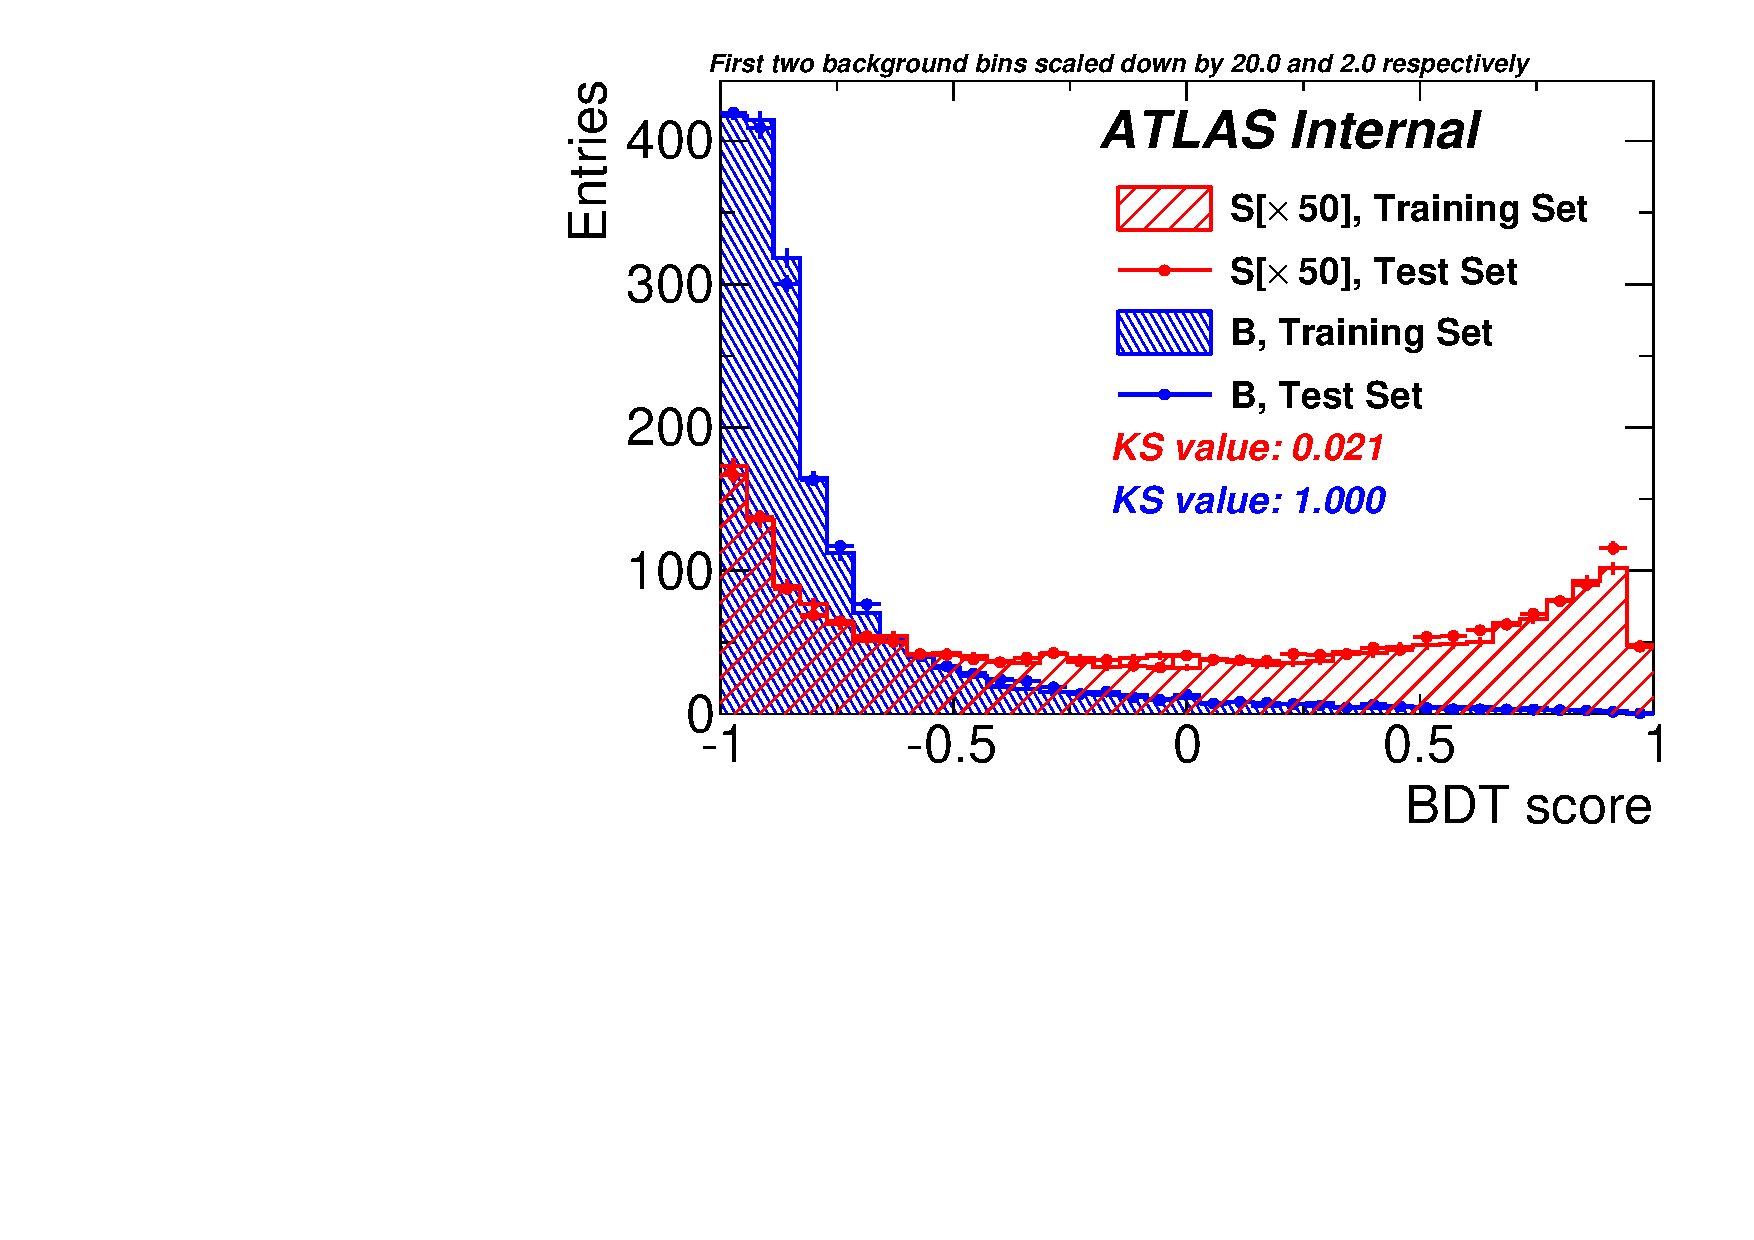
\includegraphics[width=0.6\textwidth]{bdt/overtraining_check1.pdf}
    \label{chap:analysis:fig:overtraining1}
    }
    \subfigure[Overtraining check for BDT 2]{
    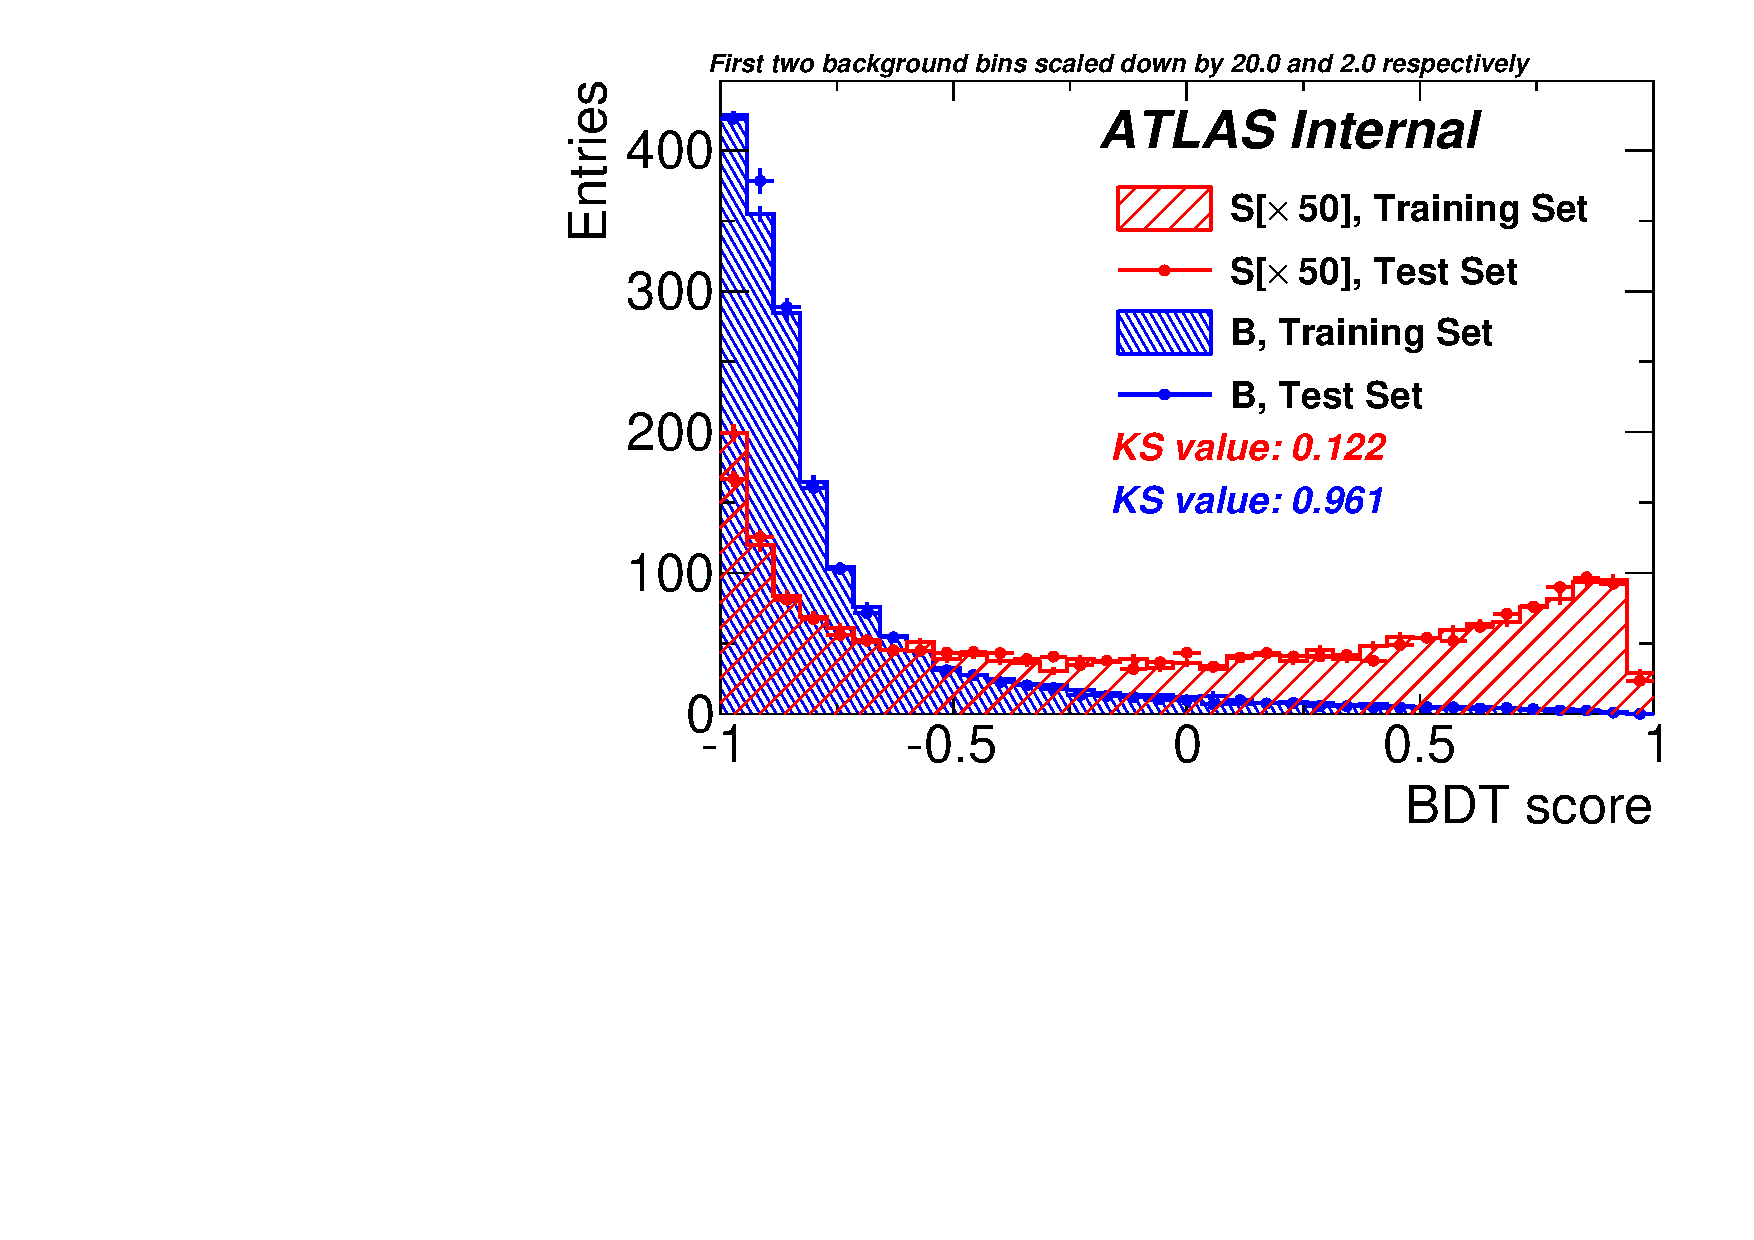
\includegraphics[width=0.6\textwidth]{bdt/overtraining_check2.pdf}
    \label{chap:analysis:fig:overtraining2}
    }
    \caption[Boosted decision tree overtraining check.]{Overtraining
      check for optimized boosted decision tree. Training set is shown
    in hatched distributions, while the statistically independent test set
    is shown with points. First two background bins are scaled by 20.0
    and 2.0, respectively. The signal normalization is multiplied by a factor
    of 50.}
\label{chap:analysis:fig:overtraining}
\end{figure}

\subsection{Data-MC Comparisons}

The BDT training relies on MC simulation to model the shapes of, and
the correlations among, the BDT inputs. In order to validate the
modelling, the level of agreement between data and MC in the BDT input
distributions is quantified in signal-depleted validation
regions. There are three such regions in this analysis: a low BDT
region, a top-rich region, and a \ZDY-rich region. The latter two will
be discussed in sections~\ref{} and~\ref{}, respectively. 

The low BDT validation region has the same preselection cuts as the signal
region, with an additional cut on the BDT score-- BDT < -0.48. The cut
value for this region has been determined through a binning optimization
algorithm for the BDT distribution. Binning optimization is performed
on the BDT distribution because the binned likelihood fit is performed
on this distribution. Hence, the statistical sensitivity of the analysis is highly
sensitive to the choice of binning. A crucial consideration in the
optimization of binning is over-fitting on statistical
fluctuations. If the metric for statistical sensitivity is not
prudently chosen, sensitivity can be arbitrarily inflated
with ever-finer binning, as backgrounds fluctuate out of signal-rich
bins. Moreover, if there is over-fitting in the binning optimization,
and bins become entirely depleted of background, then systematic
uncertainties are not properly accounted for in the fit algorithm,
again resulting in an optimistic estimate of the statistical
sensitivity. 

The binning optimization algorithm for the BDT distribution has been
chosen to account for the above considerations. First, the
preselection cuts are applied and the BDT distribution is computed for
signal at $m_{\textrm{H}} = 125$~\gev, as well as all of the
backgrounds. Because BDT peaks sharply at one for signal, the
algorithm starts at the right side of the BDT distribution, and in
BDT steps of 0.02, integrates to the left. At each step, the Poisson
significance estimate, given by

\begin{equation}
\label{chap:analysis:equation:pois_sig}
Z_{\textrm{Pois}}(S,B) = \sqrt{2((S+B)\log{(1+S/B)}-S)},
\end{equation}

\noindent
where $S$($B$) is the signal(background) event count normalized to
luminosity, is computed. When a maximum in $Z_{\textrm{Pois}}(S,B)$ is
reached, the event yield for each background is checked, and if each
background is represented, a bin boundary is set at that BDT
value. The next iteration then begins at the new boundary until another
maximum is found. The procedure continues until the maximum
$Z_{\textrm{Pois}}(S,B)$ falls below some threshold as the integration
nears the background-dominant low BDT region. The significance curves
obtained in this procedure are shown in
figure~\ref{chap:analysis:fig:bin_opt}. The resulting bin boundaries
are -0.48, 0.3, and 0.78. The region BDT~$<-0.48$ is dominated by
background (in \emme, $B \sim 660$), with little signal (in \emme, $S \sim 5$),
and is consequently not included in the signal region. Instead, this
region is used to validate the modeling of BDT inputs. 

\begin{figure}[h]
  \centering
  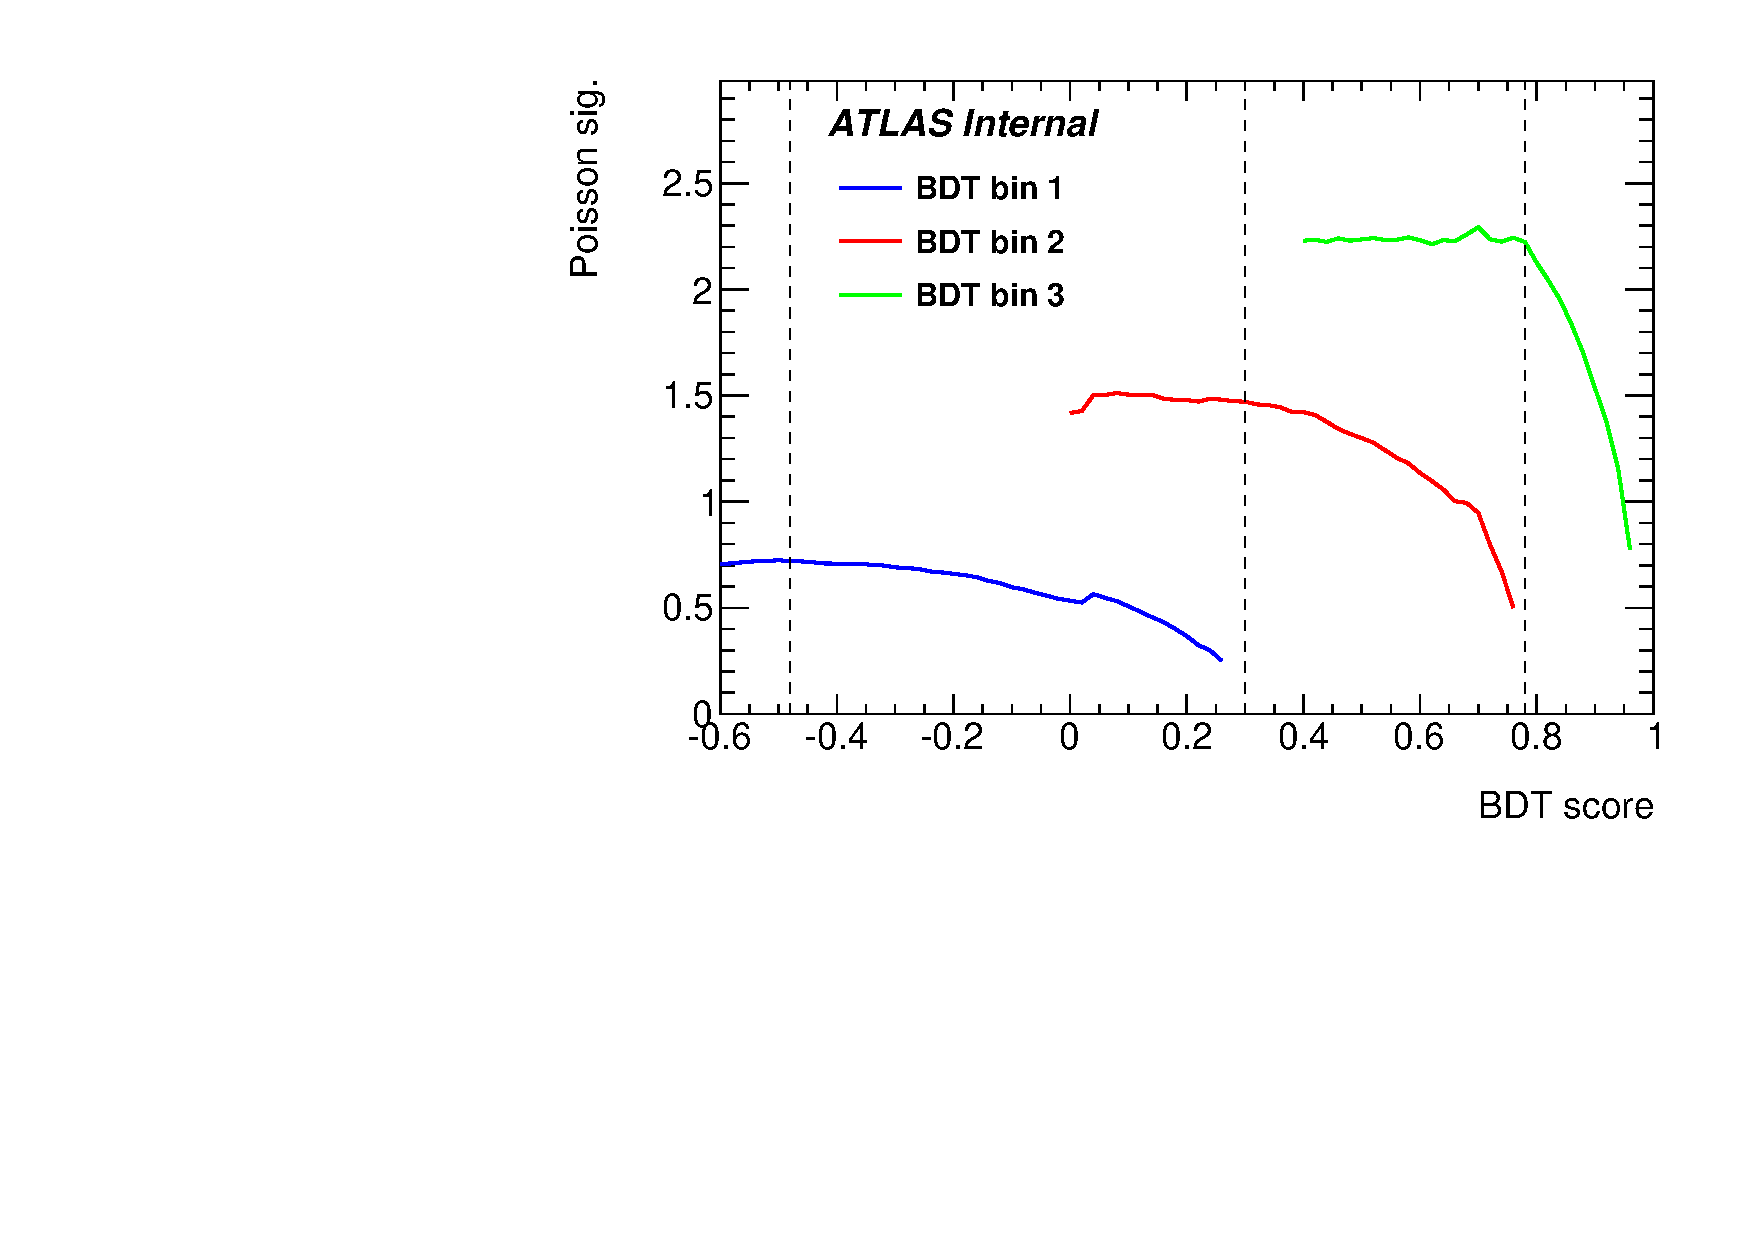
\includegraphics[width=0.6\textwidth]{fig/analysis/bin_opt_plot.pdf}
  \caption{Poisson significance scans used in the BDT bin optimization
  algorithm. Resulting bin boundaries shown as dashed lines.}
  \label{chap:analysis:fig:bin_opt}
\end{figure}

Data-MC comparisons for the eight BDT inputs in the BDT~$<-0.48$
validation region (VR) are shown in
figure~\ref{chap:analysis:fig:low_bdt_vr_df}. Despite the fact that
there are not any data-driven corrections applied to the MC
predictions in these plots, the MC models the data well in this
region, as indicated by the $p$-value from the KS test for each BDT
input. The lowest $p$-value, for \lepEtaCent, is 0.38-- less than a
one sigma discrepancy. 

\begin{figure}[h]
  \centering
  \includegraphics[width=0.4\textwidth]{fig/analysis/low_bdt_vr/emme_CutBDTScore_Bin1_DPhill_mh125_lin.eps}
   \includegraphics[width=0.4\textwidth]{fig/analysis/low_bdt_vr/emme_CutBDTScore_Bin1_Mll_mh125_lin.eps}
   \includegraphics[width=0.4\textwidth]{fig/analysis/low_bdt_vr/emme_CutBDTScore_Bin1_DYjj_mh125_lin.eps}
   \includegraphics[width=0.4\textwidth]{fig/analysis/low_bdt_vr/emme_CutBDTScore_Bin1_Mjj_mh125_lin.eps}
   \includegraphics[width=0.4\textwidth]{fig/analysis/low_bdt_vr/emme_CutBDTScore_Bin1_Pttot_tr_mh125_lin.eps}
   \includegraphics[width=0.4\textwidth]{fig/analysis/low_bdt_vr/emme_CutBDTScore_Bin1_MT_tr_mh125_lin.eps}

   \includegraphics[width=0.4\textwidth]{fig/analysis/low_bdt_vr/emme_CutBDTScore_Bin1_SumOFMvaMLepxJety_mh125_lin.eps}
   \includegraphics[width=0.4\textwidth]{fig/analysis/low_bdt_vr/emme_CutBDTScore_Bin1_contOLV_mh125_lin.eps}
   \caption{Distributions of \dphill, \mll, \dyjj, \mjj, \pTtot,  \mT,
     \SumMlj, and \lepEtaCent in the \emme VR (BDT score~$<-0.48$). }
  \label{chap:analysis:fig:low_bdt_vr_df}
\end{figure}

In addition to the one-dimensional BDT input distributions, the
modeling of the correlations among the BDT inputs has been
investigated. This is accomplished by plotting the average value of
the $i^{\textrm{th}}$ BDT input against the $j^{\textrm{th}}$ input
for all possible pairs of BDT inputs. The resulting matrix of
plots is shown in figure~\ref{chap:analysis:fig:bdt_corr_vr} for the
low BDT VR. The background color in each subplot is based on the
$p$-value for the $\chi^2$ test. If the $p$-value falls below 0.05,
the background is set to red. In this region, the MC models the correlations observed in
data well. Mismodeling in the correlations will also manifest as
data-MC discrepancies in the BDT response distribution. 

(insert plot of log(BDT) in low BDT VR.)

\begin{figure}[h!]
  \centering
  \includegraphics[width=1.0\textwidth]{fig/analysis/bdt_correlation_validation/correlations_PROF_lowBDT_VR.eps}
  \caption{Correlation plots of BDT inputs in the low BDT VR. Distributions of
    $< X_i >$ vs $X_j$ are shown for each BDT input pair. Data is
    shown in black, while the MC prediction for the background is in
    red. The background color for a given plot is set according to the
  $p$-value from the $\chi^2$ test. If the $p$-value is less than
    0.05, i.e. the discrepancy is greater than 2$\sigma$, the
    background is red. The test only accounts for statistical uncertainties.}
  \label{chap:analysis:fig:bdt_corr_vr}
\end{figure}



\section{Data-driven background estimates}
\label{chap:analysis:sec:dd_backgrounds}

As discussed in section~\ref{sec:data_mc}, background predictions are
derived from MC simulation. In some cases, the accuracy of the
prediction from simulation can be improved upon by incorporating
information from the data collected in the ATLAS detector. These
``data-driven'' approaches are summarized in the following section.

\subsection{Top Quark Processes}
\label{chap:analysis:sec:dd_backgrounds:subsec:top}
%
Top background is comprised mainly of \ttbar~(Figure), with $s$ and $t$
channel single top and $Wt$ contributions as well (denoted ST). The parton
level process for \ttbar~is simulated in
\POWHEG at NLO in QCD, while \PYTHIAns 6 is used for parton showering and
hadronization. The LO PDF set CTEQ6L1 is used with \PERUGIA 2011 as
the underlying event tune. Past iterations of the VBF analysis in this
decay channel used \MCATNLO to model
\ttbar~\cite{bib:hww_moriond_2013}, but \POWHEGns +\PYTHIA models jet
kinematic distributions better in the VBF phase space region. However, leptons generated in
\MCATNLO model the data better than \POWHEG. To account for these
modelling differences, theoretical uncertainties are assigned to the
predicted \ttbar~yield in the signal region. For ST,
$s$ channel and $Wt$ use \POWHEGns +\PYTHIAns 6 as well, while
\textsc{AcerMC}+\PYTHIAns 6 is used to model $t$-channel ST. The same PDF
and UE tune is used for all top processes. 

The \ttbar~normalization is scaled to the cross section for $pp$
collisions at \sqrts$=8$ \tev~for a top quark mass of
$172.5 \gev/c^2$, $\sigma_{t\bar{t}}=252.9^{+15.3}_{-16.3}$~pb. This value has been
calculated at NNLO in QCD including a resummation of
next-to-next-to-leading logarithmic (NNLL) soft gluon
terms~\cite{bib:Cacciari:2011hy,bib:Beneke:2011mq,bib:Baernreuther:2012ws,bib:Czakon:2012zr,bib:Czakon:2012pz,bib:Czakon:2013goa,bib:Czakon:2011xx}.
The total cross section for \ttbar~has been measured to be
$237.7\pm11.3$~pb in the leptonic decay channel with one
electron and one muon in the final
state~\cite{bib:ttbar_cross_section}, agreeing with the
theory calculation within the QCD scale uncertainties. The $s$ channel
ST, $t$ channel ST, and $Wt$ normalizations are also scaled to the
NNLO and NNLL cross sections of $5.61\pm0.22$~pb~\cite{bib:Kidonakis:2010tc},
$87.76^{+3.44}_{-1.91}$~pb~\cite{bib:Kidonakis:2011wy}, and
$22.37\pm1.52$~pb~\cite{bib:Kidonakis:2010ux}, respectively. These
computations are compatible with the respective measurements in
ATLAS~\cite{bib:tchan_cross_section,bib:Wt_cross_section}. 

In spite of the high level of agreement observed between theory
calculations and ATLAS top measurements, the top normalization is
constrained using a top-rich control region (CR). The cross section
measurements in
ATLAS,~\cite{bib:ttbar_cross_section,bib:Wt_cross_section}, require
the selected jets to be central ($|\eta|<2.5$), whereas in the VBF
analysis, due to the signal topology, the $\eta$ requirement is looser,
$|\eta|<4.5$. Dedicated top measurements have yet to probe this region
to test existing theoretical models, motivating the use of a
data-driven top estimate. Because the kinematic
shapes are similar for \ttbar~and ST, these processes share a common
normalization. All of the selection cuts applied in the SR are also
applied in the top CR, with the exception of the BJV. Instead of
requiring zero $b$-tags, exactly one $b$-tag is required, enriching
this region with top background while while minimizing contamination from
sources without heavy flavor quarks in the final state. The top CR is
subdivided into BDT bins, and the top
normalization is computed separately in each bin. This approach is
used because the BDT spans a large and relatively unknown region of
phase space, and there is no \textit{a priori} reason to assume that the
normalization is constant across the BDT spectrum. The normalization
factor in BDT bin $i$ can be expressed as

\begin{equation}
\label{chap:analysis:equation:top_nf}
NF_i = \frac{N_{data}^{CR} - N_{non-top}^{CR}}{N_{top}}
\end{equation}




%\subsection{SM $WW+2\textrm{j}$}
%
Non-resonant standard model $WW$ production is a major background to
VBF \hww: \textapprox{19\%} in the \emme SR and \textapprox{9\%} in
the \eemm SR. 


%\subsection{Gluon Fusion Higgs}
%As discussed in section XX, gluon fusion is the dominant Higgs production mode at the
LHC, with a cross section that is a factor of \textapprox{10} larger
than VBF. Requiring two jets in the final state, however, suppresses
this background significantly. Furthermore, given that the jets in ggF
events arise from QCD vertices, cuts that isolate the VBF topology
efficiently remove ggF. Nevertheless, because the it is the same Higgs
decay, there is phase space overlap between the signal and this
background, and in the \emme channel, ggF accounts for 10\% of the
total background, assuming a Higgs mass of 125 \GeV.

The ggF$+2$j process is simulated with \POWHEG interfaced with
\PYTHIAns8. The cross section is computed at NNLO in
QCD~\cite{Djouadi:1991tka,Dawson:1990zj,Spira:1995rr,Harlander:2002wh,Anastasiou:2002yz,Ravindran:2003um},
with NLO electroweak corrections~\cite{Aglietti:2004nj,Actis:2008ug}
and soft gluon resummations up to
next-to-next-to-leading-log (NNLL)~\cite{Catani:2003zt}, as recommended by
the LHC Higgs Cross Section Working
Group~\cite{bib:Dittmaier:2011ti,bib:Dittmaier:2012vm,bib:Heinemeyer:2013tqa}. The
branching fraction used in the normalization comes from
\hdecay~\cite{Djouadi:1997yw}, with the associated uncertainties
compiled
in~\cite{bib:Dittmaier:2011ti,bib:Dittmaier:2012vm}. Due
to known deficiencies in the Higgs $p_T$ spectrum in \POWHEG, the
Higgs $p_{\mathrm{T}}$ is re-weighted to the NLO + NNLL prediction
from \HqT~\cite{deFlorian:2011xf}. With these corrections, the cross
section for this decay channel is $\sigma({\hww}) =
\sigma_{\mathrm{total}}(m_H = 125)\mathrm{BR}(\hww) =
19.27~\mathrm{pb}\cdot{0.215} = 4.15$~pb.

Mention using 0,1j to constrain ggF normalization?




\subsection{\ZDYll and \Ztautau}
%
In the \eemm channel, the dominant background, \ZDY, is significantly
suppressed by requiring the events to fall at high values of
\etmiss. Processes which produce a $Z/\gamma^{*}$ in association with
jets do not have ``real'' \etmiss from invisible final state
particles. Instead, \etmiss arises due to the mismeasurement of
leptons or jets in the final state, as well as soft QCD activity from the underlying
event or pile-up. Such instrumental effects are difficult to model in
MC simulation, motivating the use of data-driven approaches. 

To correct for mismodeling of calorimeter-based \etmiss in \ZDY MC, the
efficiency of the \calomet$>45$~\gev~cut is taken from data. After
applying the common preselection cuts and the track \etmiss cut, the
\mll-\etmiss plane is partitioned into four orthogonal regions, labeled A, B, C,
and D (table~\ref{chap:analysis:tab:bdt_abcd_cartoon}). Regions C and D fall in the $Z$ peak ($|\mll -
m_Z| < 15$~\gev), with region C at high \etmiss ($>45$~\gev) and
region D at low \etmiss ($25 < $~\gev~$\etmiss$~$ <
45$~\gev). Similarly, regions A and B fall at high and low \etmiss,
respectively, but at low \mll (\mll$< 75$~\gev). In this way, region A
corresponds to the \eemm SR. Region B is rich in \ZDY, with
\textapprox{5$\%$} contamination from other backgrounds. Consequently,
data from this control region is used to obtain the \ZDY template in
region A. To extrapolate from region B to region A, the number of
events is scaled by the \etmiss efficiency from regions C and D. The
estimate in region A can be written,

\begin{equation}
\label{chap:analysis:equation:dy_est1}
N_{\mathrm{DY},i}^A = \frac{N_{\mathrm{DY},\mathrm{data}}^{C}}{N_{\mathrm{DY},\mathrm{data}}^{D}}\dot{N_{\mathrm{DY},\mathrm{data},i}^{B}}
\end{equation}

\noindent
where $N_{\mathrm{DY},\mathrm{data}}$ is the number of data events in the control
region with the non-$\mathrm{DY}$ component, predicted by MC,
subtracted. The index $i$ labels the BDT bin. The \etmiss efficiency
is not binned in BDT-- i.e. the same ratio is applied for each bin. As
for the top estimate, due to limited statistics in the high BDT bins,
the control regions for these bins are merged. Therefore, the relative
rates in these two bins are taken from the MC prediction. 

\begin{table}
\centering
%\vspace{0.5cm}
{\footnotesize
    \centering
    \begin{tabular}{|c|c|}
        \hline
        & \\
        \textbf{Region A (SR)}                          &
        \textbf{Region C }                           \\
        & \\
        $\calomet > 45 \GeV$                            & $\calomet >
        45 \GeV$                          \\
        $\mll < 75 \GeV$                                & $|\mll -
        m_Z| < 15 \GeV$              \\
        & \\
        \hline
        & \\
        \textbf{Region B}             & \textbf{Region D} \\
        & \\
        $25 \GeV < \calomet < 45 \GeV$          & $25 \GeV < \calomet
        < 45 \GeV$                        \\
        $\mll < 75 \GeV$                                & $|\mll -
        m_Z| < 15 \GeV$                      \\
        & \\
        \hline
    \end{tabular} }
\caption[Summary of the regions used for the data-driven \ZDY~estimate.]{Summary of the regions used for the data-driven
  \ZDY~estimate (ABCD method).}
\label{chap:analysis:tab:bdt_abcd_cartoon}
\end{table}

This so called ``ABCD method'' is predicated on two assumptions. The
first is that the BDT response is not correlated to calorimeter
\etmiss, allowing the BDT shape template to be taken from the low
\etmiss CR. The second implicit assumption is that the calorimeter
\etmiss cut efficiency is not correlated with \mll. This assumption
is needed to apply the low to high \etmiss extrapolation factor from
the $Z$ peak in the low \mll region. The validity of these two
assumptions is empirically tested in MC, and any breakdown is
accounted for in the assignment of systematics uncertainties. 

The absence of a correlation between the BDT response and calorimeter \etmiss
is due to the fact that jet-corrected \trkmet is used in the only two
BDT inputs that depend on \etmiss, \mT and \pTtot. The linear
correlation coefficients between the BDT inputs and both calorimeter
and track \etmiss are shown
in~\ref{chap:analysis:tab:bdt_met_corr}. With the exception of \mT,
the correlation between calorimeter \etmiss and the BDT inputs is less
than 0.1. To account for any correlation, the difference in the shape
of the BDT template in regions A and B is taken as an
uncertainty. This difference is computed in A{\sc lpgen}+H{\sc
  erwig} and A{\sc lpgen}+P{\sc ythia}, and the largest uncertainty
between the two MC generators is assigned. The template comparisons
are shown in figure~\ref{chap:analysis:fig:bdt_met_corr}, with
uncertainties corresponding to 4\%, 10\%, and 60\% in bins of BDT. 

\begin{table}[h]
\centering
\renewcommand{\arraystretch}{1.2}
%{\small
%\resizebox{0.8\textwidth}{!}
{
\begin{tabular}{| l | c | c |}
\hline
BDT input & \calomet & \trkmet \\
\hline
\mT & 0.14 & 0.31 \\
\pTtot & 0.00 & 0.07 \\
\mjj & 0.08 & 0.11 \\
\SumMlj & 0.08 & 0.10 \\
\dphill & -0.04 & 0.02 \\
\mll & 0.03 & 0.04 \\
\lepEtaCent & 0.02 & 0.00 \\
\dyjj & -0.02 & 0.05 \\
\hline
\end{tabular}
}
\caption[Linear correlation coefficients between BDT inputs and
  \etmiss quantities for \ZDY.]{Linear correlation coefficients between BDT
  inputs and \etmiss quantities for \ZDY.}
\label{chap:analysis:tab:bdt_met_corr}
\end{table}

\begin{figure}[h]
  \centering
  \includegraphics[width=0.5\textwidth]{fig/analysis/bdt_met_corr_herwig.eps}
  \includegraphics[width=0.5\textwidth]{fig/analysis/bdt_met_corr_pythia.eps}
   \caption[]{Comparison of BDT template for \ZDY in
     $25 \gev < \etmiss< 45 \gev$~region (blue) and $\etmiss >
     45 \gev$~region (red). The nominal \ZDY sample A{\sc lpgen}+H{\sc
       erwig} is shown on the left and A{\sc lpgen}+P{\sc ythia} is on
     the right.}
  \label{chap:analysis:fig:bdt_met_corr}
\end{figure}

The second assumption, that the calorimeter \etmiss efficiency is not
correlated to \mll, is true for the leading order $Z$+$2j$
processes. However, for higher order processes with ISR, the
lepton-jet system recoils against the QCD radiation, thereby
increasing \mll. The soft hadronic activity associated with ISR is
more susceptible to mismeasurement, translating to a larger calorimeter
\etmiss resolution. With larger \etmiss tails and higher \mll in ISR
events, a correlation between these two quantities is
induced. Therefore, the efficiency of the \calomet$>45$~\gev~cut in the $Z$ peak is expected
to be greater than that in the \mll$<75$~\gev~ region. The degree to
which the efficiencies disagree is referred to as the non-closure of
the method, and is quantified by

\begin{equation}
f_{\textrm{non-closure}} = \frac{N_A/N_B}{N_C/N_D}
\label{chap:analysis:equation:abcd_nonclosure}
\end{equation}

\noindent
where the event yields are taken from \ZDY MC. The \ZDY estimate in
the SR, given by equation~\ref{chap:analysis:equation:dy_est1}, is
scaled by this factor $f_{\textrm{non-closure}}$ to account for the
\etmiss efficiency difference. Moreover, the difference between
$f_{\textrm{non-closure}}$ and unity (17\%) is assigned as an
uncertainty. (discuss study of non-closure in data?). The \etmiss
efficiency in the $Z$ peak ($N_C/N_D$), as measured in data, is $0.43
\pm 0.03$, which is constitent with the value from \ZDY MC of $0.47
\pm 0.04$. The statistical uncertainty on this efficiency is taken as
an uncertainty.

There is a final uncertainty due to the fact that the relative yields
in the last two bins are taken from MC. Three sources of uncertainty
on the relative yields have been considered: (1) QCD scale, (2) parton
shower, (3) PDF. Of these three sources, evaluated with \SHERPA, the
largest is QCD scale, corresponding to an uncertainty of 11\% in the
last BDT bin. The other two sources are neglected.

The $Z$ boson processes in which the $Z$ decays to $\tau\tau$
contribute in both the \emme and \eemm channels. The normalization of
this background is taken from a control region that includes all of
the preselection cuts with the exception of the
$Z\rightarrow{\tau\tau}$ veto. Instead, $Z\rightarrow{\tau\tau}$ is
enhanced by requiring that $|\mtt - m_Z| < 25 \gev$. Additionally, the
cut $\mll < 80 \gev$~is applied to \emme events, and to pick out a
more signal-like phase space region, $\textrm{BDT} > -0.48$ is
required. In order to increase the statistics in this region, thereby
decreasing the statistical uncertainty on the NF, the \emme and \eemm
channels are merged for a common NF. The resulting NF is $0.9 \pm
0.3$. The same normalization is applied across the BDT spectrum due to
limited $Z\rightarrow{\tau\tau}$ statistics at high BDT. 


\subsection{$W+$jets and QCD}
%
Although \wjets and QCD multijet processes (figure~\ref{}) do not contain two
leptons in the final state, they are expected to contribute in the
signal region in cases where a jet is mis-reconstructed as a prompt
lepton.  Such leptons are considered ``fake'', whether they are
mis-reconstructed from charged hadron tracks or from heavy hadron
decays to true non-prompt leptons. Given that this background is due
to instrumental effects, a reliable estimate can only be obtained with
data-driven methods. In contrast to the data-driven estimates
described above, the procedure described in the following section
is purely data-driven in the sense that both the normalization and the
kinematic shapes are derived from a control region. In other words,
\wjets MC templates are not used at all.

The \wjets CR is the same as the analysis signal region except that
the object selection has been adjusted to enrich the region with fake
leptons. This is accomplished by loosening the quality criteria for
one of the leptons and requiring that it does not pass the analysis-level
lepton selection, while the other lepton is required to pass. The
former lepton type is referred to as ``anti-identified''. For
anti-identified electrons, the calorimeter isolation requirement is
loosened to $\et^{R=0.3}/\et<0.30$, the track isolation requirement
is $p_T^{R=0.3}/\et<0.16$, the conversion flag and $b$-layer
requirements are removed and the electron is required to fail the {\it
  medium} identification requirement. For muons, the calorimeter
isolation requirements are also loosened, the track isolation
requirements are completely removed, and the transverse impact parameter
significance cut is removed.

To extrapolate from the \wjets CR to the SR, first the non-\wjets
background is subtracted, and then an extrapolation factor, called the
fake factor, is applied. The fake factor is defined as

\begin{equation}
\label{chap:analysis:equation:fake_factor}
f_{\textrm{fake}} =
\frac{N_{\textrm{id}}}{N_{\textrm{anti-id}}}
\end{equation}

\noindent
where $N_{\textrm{id}}$ is the number of jets that pass the
full lepton selection and $N_{\textrm{anti-id}}$ is the number
of jets which pass the anti-identified selection. \fakefact is
evaluated with jets in a jet-rich $Z$ CR in bins of lepton \pt~and
$\eta$. From the fake factor, the \wjets estimate in the SR is given
by

\begin{equation}
\label{chap:analysis:equation:wjets_est}
N_{id+id}^{\wjets} = \fakefact\cdot (N_{\textrm{id+anti-id}} -
N_{\textrm{id+anti-id}}^{\textrm{QCD}} -
N_{\textrm{id+anti-id}}^{\textrm{non-fake,MC}})
\end{equation}

\noindent
where $N_{\textrm{id+anti-id}}$ is the total number of events in the
\wjets CR, $N_{\textrm{id+anti-id}}^{\textrm{QCD}}$ is data-driven QCD
multijet estimate in the \wjets CR, which is described below, and
$N_{\textrm{id+anti-id}}^{\textrm{non-fake,MC}}$ is the MC prediction
for the non-fake contribution in the \wjets CR. 

The dijet control region is similar to the \wjets control region,
except that instead of the requirement of one anti-identified lepton,
both of the leptons satisfy this requirement. The fake factors for
this background are obtained using the same procedure as \wjets,
except that the control region is rich in QCD dijets. Because there
are two fake leptons, two fake factors are derived, where the second
fake factor accounts for bias introduced with the requirement of an
additional anti-identified lepton. The QCD estimate in the signal
region is then expressed as

\begin{equation}
N_{id+id}^{\textrm{QCD}} = \fakefact^{\prime\prime}\cdot\fakefact^{\prime}\cdot (N_{\textrm{anti-id+anti-id}} -
N_{\textrm{anti-id+anti-id}}^{\wjets\textrm{,MC}} -
N_{\textrm{anti-id+anti-id}}^{\textrm{non-fake,MC}})
\end{equation}

\noindent
where $\fakefact^{\prime\prime}$ and $\fakefact^{\prime}$ are the two
dijet fake factors, $N_{\textrm{anti-id+anti-id}}$ is the total number
of data events in the dijet CR,
$N_{\textrm{anti-id+anti-id}}^{\wjets\textrm{,MC}}$ is the \wjets
contamination predicted by simulation in the CR, and
$N_{\textrm{anti-id+anti-id}}^{\textrm{non-fake,MC}}$ is the non-fake
contamination. 

To estimate the QCD contamination in the \wjets CR
($N_{\textrm{id+anti-id}}^{\textrm{QCD}}$ in
equation~\ref{chap:analysis:equation:wjets_est}), there is an
extrapolation from the dijet CR to the \wjets CR, given by

\begin{equation}
N_{id+anti-id}^{\textrm{QCD}} = 2\cdot\fakefact^{\prime\prime}\cdot (N_{\textrm{anti-id+anti-id}} -
N_{\textrm{anti-id+anti-id}}^{\wjets\textrm{,MC}} -
N_{\textrm{anti-id+anti-id}}^{\textrm{non-fake,MC}})
\end{equation}

\noindent
where the factor of two arises due to the fact that events with two
anti-identified leptons can enter the \wjets CR if either lepton is
identified. 

Backgrounds due to fakes are relatively small in the BDT signal
region. The primary reason for this is that the jets in \wjets and QCD
processes tend to be more central in rapidity, but the BDT selects a
region of phase space with forward jets. The \wjets estimate in the
\emme channel relative to the total background prediction is 2\%, 3\%,
and 0\%, in the respective BDT fit bins and the QCD estimate is even
smaller-- 0.4\%, 0\%, and 0\%. 

\noindent Systematics go here or later?



\section{Systematic Uncertainties}
\label{chap:analysis:sec:systematics}
All Monte-Carlo-based predictions rely on the best estimate for a set
of parameters $\hat{\vect{\theta}}$. These parameters can be
theoretical in nature, such as the cross section to which the
prediction is scaled, or intrinsic to the ATLAS detector, such as the
efficiency for selecting an electron. The uncertainties on these
parameters are propagated to uncertainties on event yields in the
signal and control regions, and as we will see in the following
chapter, these uncertainties are ultimately propagated to an error on
the measured VBF signal strength. Uncertainties are always computed at a
working point corresponding to $\pm 1\sigma$ and propagated to the
statistical fit as such.

\subsection{Theoretical sources}

Monte Carlo generators are approximate models for any scattering
process. To assess theoretical uncertainties, approximations are
varied, and the resulting change in the prediction is
quantified. The following sources of uncertainty are considered:
parton distribution function (PDF), QCD scale, parton showering
program, hard-scattering program, and underlying event tune. Depending
on the source, these uncertainties are split into two kinds:
normalization and acceptance. Normalization uncertainties are those
that vary the overall normalization of a prediction without changing
the underlying distributions. Acceptance uncertainties are computed
for sources that change kinematic distributions and therefore
selection efficiences. Because the BDT spectrum spans a large and
relatively unknown region of phase space, acceptance uncertainties are
computed separately in each BDT fit bin.

Varying the factorization ($\mu_F$) and renormalization scales
($\mu_R$) probes sensitivity to the corrections from the next order in
the perturbative expansion. For the VBF process, $\mu_F$ and $\mu_R$
are varied up and down by a factor of two, and the resulting change in
event rates in the signal region is on the order of 0.5\%. Since the
scale change impacts the BDT input distributions associated with tag
jets, namely \mjj and \dyjj, there is a distortion of the BDT
spectrum of [1\%,3\%,3\%] in BDT bins. 

The PDF uncertainty is also evaluated for the VBF signal process. 
Comparing the baseline PDF \ctten to \nnpdf (reference), the
difference in event yields in the BDT SR is found to be 4\%, with a
negligible dependence on the BDT score. The baseline hard-scattering
generator is \POWHEG which simulates the VBF process at NLO in
QCD. Another generator, \aMCATNLO, utilizes a different prescription
for matching the HS and the PS, and in order to ascertain the
uncertainty associated with the default prescription, the predictions
of the two generators are compared. Although the shape variation of
the BDT distribution is negligible, \aMCATNLO predicts 4\% more events
than \POWHEG in the BDT SR, which is assigned as a normalization
uncertainty. Additionally, uncertainties associated with corrections
from higher order EW corrections are assessed by turning these
corrections on and off in the generator \VBFNLO. These corrections are
observed to have little impact on the shape of the BDT spectrum, and
increase the overall cross section by 3.5\%, a correction which is
already accounted for in the NLO cross section calculation to which
the baseline prediction is scaled~\ref{chap:analysis:sec:data_mc}.

The dominant uncertainty on signal is associated with the parton
shower program. Comparing the baseline program \PYTHIA is to \HERWIG,
the difference in the event yield in the signal region is 3.4\%. The
distortion of the BDT spectrum is large due to the fact that a BDT
input, \pttot, shown in figure~\ref{}, is highly sensitive to the soft
jet activity in an event. Though the effect is as large as 50\% in
the \pttot distribution, in the BDT distribution the largest
difference is 10\% in the highest BDT bin, because the BDT selects the
region of phase space associated with the core of the \pttot
distribution. 

As discussed in
section~\ref{chap:analysis:sec:dd_backgrounds:subsec:top}, the
theoretical uncertainties
for \ttbar and ST are computed by varying the PDF, QCD scale, parton
shower, and the hard-scattering generator. Because this background is
normalized with a control region, the change in the extrapolation
factor $\alpha = \frac{N_{top,MC}^{SR}}{N_{top,MC}^{CR}}$
(equation~\ref{chap:analysis:equation:top_est}) is measured in order to
assess the uncertainty on the signal region event rate. The dominant
uncertainty source has been found to be the hard-scattering generator,
derived from a comparison of \MCATNLO and \ALPGEN. In the respective
BDT fit bins, these uncertainties are 10\%, 12\%, and 21\%.

Non-resonant \wwtwoj production is a large background,
contributing \textapprox{19\%} in the \emme SR and \textapprox{9\%} in
the \eemm SR. QCD \wwtwoj rates are predicted with an
inclusive \SHERPA sample normalized to the NLO \MCFM cross section. To
assess the hard-scattering and QCD scale uncertainties, \MADGRAPH interfaced
with \PYTHIA 6 for showering is used. The sample which is generated is
also inclusive, with up to three partons generated at the matrix
element
level. These final state partons are then showered in \PYTHIA with the
MLM matching scheme (reference) at a scale of 20~\gev. The PDF in
both \MADGRAPH and \PYTHIA is \cteqsixl, and the underlying event tune
is AUET2B (reference). 

The hard-scattering uncertainty is computed by comparing
the truth level predictions of \MADGRAPH to those of the \SHERPA. In
an approach similar to the one used in the evaluation of top theory
uncertainties (section~\ref{chap:analysis:section:top}), the BDT inputs are
evaluated at truth level, and the resulting distortion of the BDT
spectrum is taken as an uncertainty. For the comparison, the two truth level
samples are scaled to the integrated luminosity with their respective
cross sections. The inclusive \MADGRAPH cross section computed after showering
is 4.55~pb, which is significantly smaller than the cross section to
which the \SHERPA prediction is scaled: 5.679~pb. However, because the
fraction of events with two or more jets is larger in \MADGRAPH, the
uncertainty after requiring two jets is mitigated. Displayed in
figure~\ref{chap:analysis:fig:qcdww_gen_uncert} is the truth level BDT
response. In light of the differences, uncertainties of 14\%, 8\%, and
12\% are assigned.

\begin{figure}[h]
    \centering
    \subfigure[QCD \ww]{
    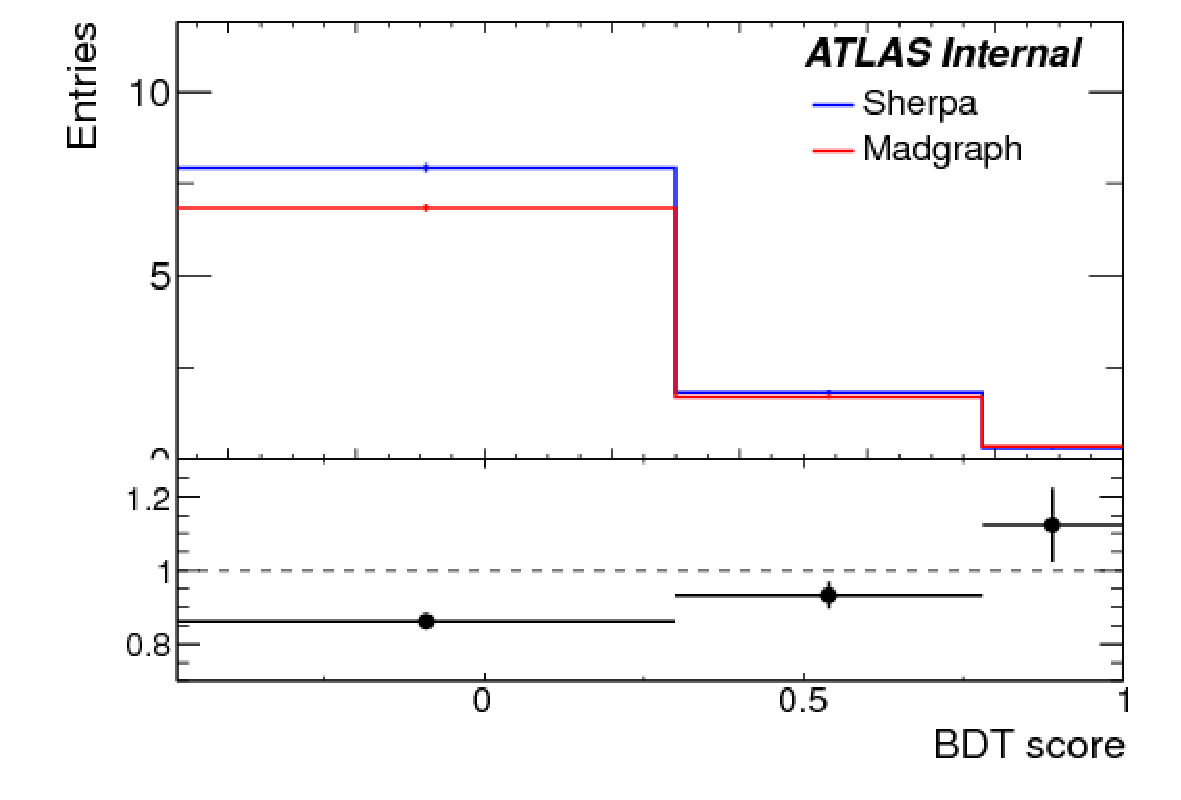
\includegraphics[width=0.45\textwidth]{analysis/ww/ww_shape_sys_qcd.pdf}
    \label{chap:analysis:fig:qcdww_gen_uncert}
    }
    \subfigure[EW \ww]{
    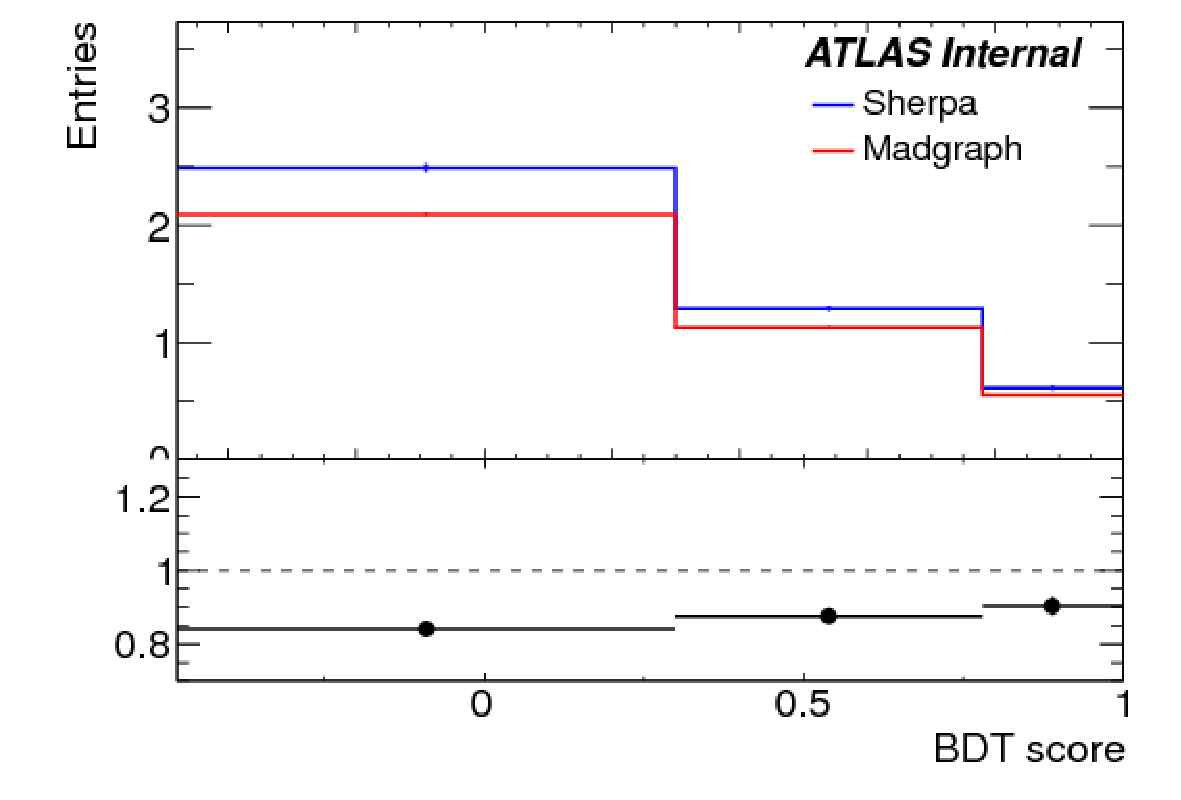
\includegraphics[width=0.45\textwidth]{analysis/ww/ww_shape_sys_ew.pdf}
    \label{chap:analysis:fig:ewww_gen_uncert}
    }
    \caption[Comparison of \MADGRAPH and \SHERPA predictions
    for \ww.]{Comparison of \MADGRAPH and \SHERPA predictions
    for \ww.}
\label{chap:analysis:fig:ww_gen_uncert}
\end{figure}

To assess the uncertainty from the choice of QCD scale, the
factorization and renormalization scales in \MADGRAPH,
which are varied dynamically event-by-event, are coherently scaled up
and down by a factor of two. The resulting samples are scaled to their
respective post-parton-showering cross sections, and the signal region
differences are computed. With the scale set to 
$\mu_R=\mu_F=\mu_{\textrm{default}}/2$, the
predicted number of events in the SR is $27\%$ higher than the default
scale choice, while with $\mu_R=\mu_F=2\mu_{\textrm{default}}$, the
prediction
falls by $2.6\%$. The larger of the two, $27\%$, is assigned as the
uncertainty, which is consistent with the LO $\sigma(WW)$
uncertainty computed at \sqrts$=7$~\tev ~\cite{bib:Melia:2011dw}, though in a
looser phase space region. Because the QCD scale variations induce
small shape differences in the BDT input distributions, the
uncertainty is flat across the BDT fit bins. Additional QCD \ww uncertainties are
summarized in table~\ref{chap:analysis:tab:ww_theory_uncerts}.

\begin{table}
\begin{center}
\renewcommand{\arraystretch}{1.2}
%\resizebox{0.8\textwidth}{!}{
    \begin{tabular}{ l | c | c }
    \hline
    Source & QCD \ww & EW \ww \\
    \hline \hline
    Generator modeling & (12\%,8\%,12\%) & (16\%,12\%,10\%) \\
    QCD scale & 27\% & 10\% \\
    PDF ($\sigma$) & 4\% & 3\% \\
    PDF (acceptance) & 2\% & $-$ \\
    QCD-EW interference & $-$ & 2\% \\
    Higgs interference & $-$ & 1.2\% \\
    \hline
    \end{tabular}
%}
\caption[Summary of \ww~theory uncertainties.]{Summary of \ww~theory
    uncertainties.}
\label{chap:analysis:tab:ww_theory_uncerts}
\end{center}
\end{table}

For EW \ww, a hard-scattering modeling uncertainty is computed by comparing
the prediction of \SHERPA to that of an exclusive two jet \MADGRAPH
sample interfaced
with \PYTHIA. The cross section computed in \MADGRAPH is 27.37~fb,
30\% lower than that of \SHERPA, resulting in fewer events
predicted. A comparison of the absolute predictions for the two
generators is shown in
figure~\ref{chap:analysis:fig:ewww_gen_uncert}, corresponding to
uncertainties of 16\%, 12\%, and 10\% in BDT bins.

The QCD scale uncertainty is computed at LO
in~\cite{bib:Jager:2006zc}. The uncertainty is computed in a generic
VBF phase space region with cuts on \dyjj and \mjj. Such a region is
expected to significantly overlap with the SR defined by the BDT. The
resulting uncertainty, computed by varying $\mu_F$ and extracting the
cross section, is 10\%.

Remaining theory uncertainties for EW \ww are shown in
table~\ref{chap:analysis:tab:ww_theory_uncerts}. The uncertainty from
interference
between EW \ww and Higgs-mediated \ww is computed by comparing the
cross section of \ww and \hww diagrams without interference to the
corresponding cross section with interference. At a Higgs mass
hypothesis of $m_H = 125$~\gev, the uncertainty is 1.2\%, while at
$m_H = 150$~\gev, the uncertainty is 6.4\%. Because these are small
with respect to the modeling and QCD scale uncertainties, they are
neglected in the fit. An uncertainty due to interference between QCD
and EW \ww processes is evaluated in a similar way and found to
be \textapprox{2\%}. This, too, is neglected in the fit.

Gluon-gluon-fusion Higgs production (ggF) is a large background in the
most sensitive BDT bins. In order to estimate the uncertainties from
higher order terms in the perturbative expansion, the $\mu_F$ and
$\mu_R$ are independently varied in \MCFM. Since the final statistical
result is derived from a likelihood across the jet bins, it is
important to correctly correlate the normalization uncertainty for
each jet bin. Moreover, applying a central jet veto effectively limits
the phase space to the exclusive two jet bin, calling for the
uncertainty to be computed for such a region. An approach that
accounts for these considerations has been proposed by Stewart and
Tackmann~\ref{bib:Stewart:2011cf}. The exclusive cross section can be
expressed as 

\begin{equation}
\sigma_{\textrm{2j}} = \sigma_{\geq\textrm{2j}} - \sigma_{\geq\textrm{3j}}
\end{equation}

where $\sigma_{\geq\textrm{2j}}$ ($\sigma_{\geq\textrm{3j}}$) is the
inclusive two (three) jet cross section. To a good approximation,
$\sigma_{\geq\textrm{2j}}$ and $\sigma_{\geq\textrm{3j}}$ can be
considered to be uncorrelated, and therefore the uncertainty on the
exclusive two jet cross section can be computed as the quadrature sum
of the two inclusive uncertainties. To ascertain the uncertainties
in \MCFM, the scales are varied, and the BDT preselection is
applied. For the inclusive 2j bin, the CJV is not applied, and for the
inclusive 3j bin, the CJV is inverted. The resulting relative
uncertainties are $\Delta_{\geq\textrm{2j}} = 22\%$ and
$\Delta_{\geq\textrm{3j}} = 118\%$, corresponding to a normalization
uncertainty of $\Delta_{\textrm{2j}} = 34\%$ in the BDT signal
region. In addition, the shape variation with QCD scale is computed
and found to be [+2.4/-2.5,+2.6/-2.5,+13/-12]\% in the BDT fit
bins. 

Uncertainties on ggF from other sources are small with respect to the
QCD scale uncertainty. The PDF uncertainty is 8\%. The underlying
event and parton shower uncertainty, computed by comparing \HERWIG
showering to the baseline program \POWHEG, is a flat 15\% across the
BDT bins. 

For \ZDYll processes, because a data-driven approach is used, the only
prediction from MC simulation is the relative rate in the last two BDT
bins. Three sources of uncertainty
on this quantity have been considered: (1) QCD scale, (2) parton
shower, (3) PDF. Of these three sources, evaluated with \SHERPA, the
largest is QCD scale, corresponding to an uncertainty of 11\% in the
last BDT bin. The other two sources are neglected. In the \emme
channel, the \Ztautaunody normalization is constrained from a control
region, which, due to limited statistics in this region, results in a
large statistical uncertainty of 30\%. Due to the negligible
contribution of this background in the most sensitive BDT bins and to
the fact that the theory uncertainties are {\it a priori} assumed to
be smaller than the statistical uncertainties, theory uncertainties
are not computed for this background component. 

The theory uncertainties for the remaining backgrounds, which are
small in the SRs, will not be discussed here, as they have little
impact on the statistical result. 

\subsection{Instrumental sources}

\begin{table}[h!]
\begin{center}
\renewcommand{\arraystretch}{1.2}
\resizebox{1.0\textwidth}{!}{
\begin{tabular}{l || c c | c c c c c c }
\hline
Uncertainty & \multirow{2}{*}{Signal} & Total &
\multirow{2}{*}{top} & \multirow{2}{*}{$WW$} & \multirow{2}{*}{ggF} &
Non-$WW$ & \multirow{2}{*}{\ZDY} & \multirow{2}{*}{Fakes} \\
Source & & Back & & & & Diboson & & \\
\hline
$\textrm{Trigger}$ & 0.5 & 0.5 & 0.5 & 0.5 & 0.5 & 0.8 & 0.6 & - \\
$\textrm{electron SF}$ & 0.8 & 0.8 & 0.8 & 0.9 & 0.9 & 1.1 & 1.1 & -
\\
$\textrm{electron reso.}$ & 0.1 & 0.5 & 0.2 & - & - & 1.5 & 4.7 & - \\
$\textrm{electron scale}$ & 0.2 & 0.5 & 0.6 & 0.5 & 0.3 & 1.6 & 2.7 &
- \\
$\textrm{electron iso.}$ & 0.7 & 0.6 & 0.7 & 0.7 & 0.8 & 0.8 & 0.8 & -
\\
$\textrm{muon SF}$ & 0.3 & 0.3 & 0.3 & 0.3 & 0.3 & 0.3 & 0.3 & - \\
$\textrm{muon reso.}$ & 0.1 & - & 0.2 & 0.1 & 0.1 & 0.1 & 0.4 & - \\
$\textrm{muon scale}$ & - & 0.1 & 0.1 & 0.2 & - & - & 0.4 & - \\
$\textrm{muon iso.}$ & 0.8 & 0.7 & 0.8 & 0.8 & 0.8 & 0.9 & 0.9 & - \\
$\textrm{JES flavor}$ & 0.8 & 0.9 & 0.7 & 2.8 & 3.0 & 3.5 & 0.3 & - \\
$\textrm{JES}~\eta~\textrm{model}$ & 2.8 & 4.7 & 3.9 & 10.2 & 5.9 &
1.3 & 6.6 & - \\
$\textrm{JES}~\eta~\textrm{stat.}$ & 0.4 & 0.8 & 0.9 & 1.3 & 0.8 & 1.8
& 0.2 & - \\
$\textrm{JES flav. response}$ & 0.7 & 0.3 & 0.2 & 2.1 & 1.9 & 2.9 &
4.7 & - \\
$\textrm{JES detector}$ & 0.3 & 0.7 & 1.1 & 0.9 & 0.7 & 0.9 & - & - \\
$\textrm{JES pileup}~\pt$ & - & 0.6 & 0.2 & 0.6 & 0.3 & 0.1 & 4.3 & -
\\
$\textrm{JES high}~\pt$ & - & 0.5 & - & - & - & - & 3.8 & - \\
$\textrm{JES pileup}~\rho$ & 0.4 & - & 0.5 & 1.5 & 1.4 & 0.6 & 5.6 & -
\\
$\textrm{JES modelling}$ & 1.1 & 1.7 & 1.9 & 3.9 & 3.4 & 5.4 & 2.6 & -
\\
$\textrm{JES}~\left \langle \mu \right \rangle$ & - & 0.5 & 0.3 & 0.4
& 0.6 & 2.5 & 0.5 & - \\
$\textrm{JES}~\nvtx$ & 0.1 & 0.3 & 0.2 & 0.7 & 0.7 & 2.8 & 3.2 & - \\
$\textrm{JES AFII}$ & - & - & - & - & - & - & - & - \\
$b\textrm{-tag SF}$ & - & 2.4 & 6.5 & 0.1 & - & - & - & - \\
$\textrm{light tag SF}$ & 1.3 & 1.3 & 1.2 & 1.7 & 1.9 & 1.8 & 1.6 & -
\\
$c\textrm{-tag SF}$ & 0.4 & 0.2 & 0.2 & 0.3 & 0.2 & 0.3 & 0.2 & - \\
$\calomet~\textrm{scale}$ & - & 0.3 & - & - & - & - & 2.2 & - \\
$\calomet~\textrm{reso.}$ & - & - & - & - & - & - & - & - \\
$\trkmet~\textrm{scale}$ & 0.3 & 2.2 & 2.6 & 2.0 & 1.0 & 0.3 & 6.6 & -
\\
$\trkmet~\textrm{reso.}$ & 0.6 & 3.6 & 4.1 & 1.4 & 2.2 & 15.7 & 9.0 &
- \\
$\textrm{di-jet fake rate}$ & - & 1.9 & - & - & - & - & - & 14.5 \\
$\textrm{fake rate}~\mu$ & - & 1.6 & - & - & - & - & - & 12.0 \\
$\textrm{fake rate}~e$ & - & 2.2 & - & - & - & - & - & 17.1 \\
$\left \langle \mu \right \rangle~\textrm{re-scale}$ & 1.2 & 0.5 & 0.8
& 0.4 & 0.9 & 3.6 & 4.4 & - \\
\hline
\end{tabular}
}
\caption[Instrumental uncertainty summary in the \emme
  channel.]{Instrumental uncertainty summary in the \emme channel.}
\label{chap:analysis:tab:exp_sys_df}
\end{center}
\end{table}


\begin{table}[p!]
\begin{center}
\renewcommand{\arraystretch}{1.2}
\resizebox{0.9\textwidth}{!}{
\begin{tabular}{l || c c | c c c c c c }
\hline
Uncertainty & \multirow{2}{*}{Signal} & Total &
\multirow{2}{*}{top} & \multirow{2}{*}{$WW$} & \multirow{2}{*}{ggF} &
Non-$WW$ & \multirow{2}{*}{\ZDY} & \multirow{2}{*}{Fakes} \\
Source & & Back & & & & Diboson & & \\
\hline
$\textrm{Trigger}$ & 1.2 & 0.5 & 1.1 & 1.2 & 1.2 & 0.6 & 0.1 & - \\
$\textrm{electron SF}$ & 0.6 & 0.3 & 0.6 & 0.7 & 0.6 & 1.9 & 0.1 & -
\\
$\textrm{electron reso.}$ & - & 0.4 & 0.5 & 0.1 & 0.3 & 0.3 & 0.5 & -
\\
$\textrm{electron scale}$ & - & 0.1 & 0.1 & 1.0 & - & 3.4 & 0.2 & - \\
$\textrm{electron iso.}$ & 0.6 & 0.3 & 0.5 & 0.6 & 0.6 & 1.4 & 0.1 & -
\\
$\textrm{muon SF}$ & - & - & - & - & - & - & - & - \\
$\textrm{muon reso.}$ & - & 0.1 & - & 0.4 & - & - & 0.1 & - \\
$\textrm{muon scale}$ & - & - & 0.2 & - & - & - & 0.1 & - \\
$\textrm{muon iso.}$ & 1.0 & 0.4 & 1.0 & 1.0 & 1.0 & 0.4 & 0.1 & - \\
$\textrm{JES flavor}$ & 1.9 & 1.1 & 0.6 & 4.4 & 4.0 & 18.0 & 0.1 & -
\\
$\textrm{JES}~\eta~\textrm{model}$ & 5.2 & 3.2 & 5.4 & 9.8 & 8.0 &
10.2 & 1.2 & - \\
$\textrm{JES}~\eta~\textrm{stat.}$ & 0.6 & 0.6 & 0.9 & 1.1 & 0.6 & 4.7
& 0.3 & - \\
$\textrm{JES flav. response}$ & 1.4 & 0.9 & 0.7 & 2.3 & 2.5 & 14.2 &
0.1 & - \\
$\textrm{JES detector}$ & 0.9 & 0.7 & 1.0 & 0.6 & 0.8 & 7.4 & 0.3 & -
\\
$\textrm{JES pileup}~\pt$ & - & 0.4 & - & 0.1 & 0.3 & 0.9 & 0.6 & - \\
$\textrm{JES high}~\pt$ & - & 0.2 & - & - & - & - & 0.3 & - \\
$\textrm{JES pileup}~\rho$ & 0.4 & 0.5 & 0.1 & 2.0 & 1.0 & 10.9 & - &
- \\
$\textrm{JES modelling}$ & 2.1 & 1.6 & 1.4 & 4.6 & 4.2 & 15.2 & 0.6 &
- \\
$\textrm{JES}~\left \langle \mu \right \rangle$ & - & 0.5 & 0.1 & 1.1
& 0.7 & 3.3 & 0.4 & - \\
$\textrm{JES}~\nvtx$ & - & 0.4 & 0.1 & 1.1 & 0.3 & 7.0 & 0.3 & - \\
$\textrm{JES AFII}$ & - & - & 0.1 & - & - & - & - & - \\
$\textrm{JER}$ & 2.5 & 1.5 & 1.8 & 4.1 & 1.0 & 1.2 & 1.3 & - \\
$b\textrm{-tag SF}$ & - & 1.3 & 6.8 & - & - & 0.8 & - & - \\
$\textrm{light tag SF}$ & 1.4 & 0.6 & 1.2 & 1.8 & 2.0 & 1.3 & 0.1 & -
\\
$c\textrm{-tag SF}$ & - & - & - & 0.1 & - & 0.2 & - & - \\
$\calomet~\textrm{scale}$ & - & 0.2 & - & - & - & 3.6 & 0.2 & - \\
$\calomet~\textrm{reso.}$ & - & 0.2 & - & - & - & 5.9 & 0.1 & - \\
$\trkmet~\textrm{scale}$ & 0.1 & 1.0 & 3.0 & 1.1 & 1.1 & 2.7 & 0.6 & -
\\
$\trkmet~\textrm{reso.}$ & 0.6 & 0.9 & 1.6 & 1.2 & 1.1 & 10.1 & 0.4 &
- \\
$\textrm{di-jet fake rate}$ & - & 0.1 & - & - & - & - & - & 4.9 \\
$\textrm{fake rate}~\mu$ & - & 0.3 & - & - & - & - & - & 12.6 \\
$\textrm{fake rate}~e$ & - & 0.3 & - & - & - & - & - & 13.7 \\
$\left \langle \mu \right \rangle~\textrm{re-scale}$ & 3.4 & 0.6 & 0.4
& 1.2 & 1.7 & 13.5 & 0.2 & - \\
\hline
\end{tabular}
}
\caption[Instrumental uncertainty summary in the \eemm
  channel.]{Breakdown of the relative instrumental uncertainties (\%) in the \eemm
  channel. Uncertainties are defined as the change in the event yield
  in the BDT SR. Given that \ZDYll is data-driven, instrumental
  uncertainties do not contribute. Non-zero \ZDY uncertainties in the
  table are from the EW contribution.}
\label{chap:analysis:tab:exp_sys_sf}
\end{center}
\end{table}


\input{tex/vbf_bdt_analysis/sys_table_ee_old}
\input{tex/vbf_bdt_analysis/sys_table_mm_old}

Notes and questions about the experimental uncertainty table:
Why does trigger uncertainty double for SF?
Electron scale uncertainty is 0 for ZDY in SF, but the JES uncertainty
is large. Is electron scale uncertainty being propagated to JES?
Q: what is the percentage of mm events in SF? 58\%
Why does mu re-scaling impact SF more than DF?
What's with the JES systematics? Why are they so much larger for SF?
Is increase in JES systematic being driven by ee?


\section{Results}
\label{chap:analysis:sec:results}

The observed number of events recorded in the ATLAS detector in the
signal regions are compared to the
predictions from MC simulation and associated data-driven
approaches. An excess over the background prediction in the absence
of VBF signal, if statistically significant, is considered to be
associated with VBF Higgs production. In the following chapter, the
statistical evaluation of such a scenario is considered, and in this
section, the event yields and kinematic plots in the SRs are presented. 

Table~\ref{chap:analysis:tab:signal_region_cutflow} shows the
predicted event yields for signal and backgrounds and the observed
event yields for each cut stage in the analysis, starting at the
common pre-selection. After the common pre-selection cuts and the
requirement of two or more jets, the the expected number of VBF events in
the \emme lepton channel is 64, with a background prediction of
\textapprox{60k} events. Applying the additional VBF pre-selection
cuts, BJV, CJV, OLV, and the $Z\rightarrow{\tau\tau}$ veto, the
background contribution is significantly suppressed to 703 events,
with 17 expected signal events. The discriminating power of the BDT is
illustrated by the $\textrm{BDT} > -0.48$ cut which removes 94\% of
the remaining background, while preserving 70\% of the signal. In this
region an excess over the background hypothesis is observed, with 57
events observed and 44 expected. This excess is concentrated in the
two highest BDT bins, where the expected $S/B$ is
largest(figure ~\ref{chap:analysis:fig:bdt_response_df}). In the
first BDT bin, there is a deficit with respect to the background
prediction, due to the large correction of $1.58 \pm 0.10$ applied to
the top background in this bin. The source of this large correction is
poor lepton modeling in \POWHEG
(section~\ref{chap:analysis:sec:dd_backgrounds:subsec:top}), which is
covered by the modeling systematic. In the \eemm channel, there is
also an excess in the SR, with 54 background events and 73 events
observed. The signal prediction in this region is 6 events. Again, the
relative excess in the most sensitive BDT bins is more pronounced
(figure~\ref{chap:analysis:fig:bdt_response_sf}). 

\begin{figure}[h]
    \centering
    \subfigure[\emme channel]{
    \includegraphics[width=0.6\textwidth]{analysis/bdt_response_df_prefit.eps}
    \label{chap:analysis:fig:bdt_response_df}
    }
    \subfigure[\eemm channel]{
    \includegraphics[width=0.6\textwidth]{analysis/bdt_response_sf_prefit.eps}
    \label{chap:analysis:fig:bdt_response_sf}
    }
    \caption[BDT response distributions.]{BDT response distribution in
    ~\subref{chap:analysis:fig:bdt_response_df} \emme channel and
    ~\subref{chap:analysis:fig:bdt_response_sf} \eemm channel. The
    error band represents instrumental, theoretical and statistical
    uncertainties. Top and \ZDY normalization factors are applied. VBF
    signal is shown in hatched red, not to be confused with ggF, shown
    in solid red.}
\label{chap:analysis:fig:bdt_response}
\end{figure}

The BDT input distributions in the \emme (\eemm) SR are shown in
figure~\ref{chap:analysis:fig:bdt_inputs_sr_df}
(\ref{chap:analysis:fig:bdt_inputs_sr_sf}). These figures illustrate
that the excess in data lies in kinematic regions coincident with VBF,
most notably at high \mjj, low \dphill, low \mll, and low \pttot. 

\begin{table}[h]
\begin{center}
\renewcommand{\arraystretch}{1.2}
\resizebox{1.0\textwidth}{!}{
%\begin{tabular}{ +l^| c^ c^ c^ | c^ c^ c^ c^ c^ c }
\begin{tabular}{l || c c c | c c c c c c }
\hline
% & & & Total & & & & Non-$WW$ & & \\
\multirow{2}{*}{Cut stage} & \multirow{2}{*}{Observed} &
\multirow{2}{*}{Signal} & Total &
\multirow{2}{*}{top} & \multirow{2}{*}{$WW$} & \multirow{2}{*}{ggF} &
Non-$WW$ & \multirow{2}{*}{\ZDY} & \multirow{2}{*}{Fakes} \\
 & & & Back & & & & Diboson & & \\
\hline
$\Njet \geq 2$ & $676470$ & $134$ & $669892$ & $106081$ & $2779$ &
$198$ & $1553$ & $556559$ & $2722$ \\
\hline
$\boldsymbol{\emme~\textrm{{\bf channel}}}$ & $61434$ & $64$ & $59597$ & $53196$ & $1423$
& $103$ & $378$ & $3356$ & $1142$ \\
\ $\Nbjet = 0$ & $7818$ & $47$ & $7569$ & $3232$ & $1036$ & $76$ & $272$
& $2460$ & $493$ \\
\ $\textrm{CJV}$ & $6313$ & $40$ & $6097$ & $2462$ & $859$ & $61$ &
$226$ & $2083$ & $408$ \\
\ $\textrm{OLV}$ & $1264$ & $23$ & $1273$ & $543$ & $156$ & $18$ & $46$
& $435$ & $76$ \\
\ $Z\rightarrow{\tau\tau}~\textrm{veto}$ & $718$ & $17$ & $703$ & $370$
& $101$ & $14$ & $31$ & $134$ & $53$ \\
\ $\textrm{BDT} > -0.48$ & $57$ & $12$ & $44$ & $16$ & $9$ & $5$ & $3$ &
$5$ & $6$ \\
\hline
\ {\bf\color{blue} BDT bin 1} & $37$ & $4.4 \pm 0.1$ & $42.3 \pm 2.2$ & $21.1$
& $6.0$ & $3.0$ & $2.6$ & $4.5$ & $5.1$ \\
\ {\bf\color{blue} BDT bin 2} & $14$ & $4.3 \pm 0.1$ & $7.9 \pm 0.9$ & $2.6$ &
$2.1$ & $1.2$ & $0.8$ & $0.6$ & $0.7$ \\
\ {\bf\color{blue} BDT bin 3} & $6$ & $3.1 \pm 0.1$ & $1.5 \pm 0.2$ & $0.4$ &
$0.5$ & $0.3$ & $0.1$ & $0.2$ & $0.0$ \\
\hline
$\boldsymbol{\eemm~\textrm{{\bf channel}}}$ & $615036$ & $70$ & $607896$ & $50497$ &
$1356$ & $95$ & $1175$ & $553203$ & $1569$ \\
\ $\calomet > 45 \gev$ & $119456$ & $45$ & $118395$ & $38710$ & $1025$ &
$60$ & $736$ & $77376$ & $488$ \\
\ $\trkmet > 40 \gev$ & $58672$ & $39$ & $56435$ & $35832$ & $944$ &
$51$ & $640$ & $18560$ & $408$ \\
\ $Z~\textrm{veto}$ & $34339$ & $35$ & $33174$ & $28358$ & $756$ & $50$
& $177$ & $3509$ & $323$ \\
\ $\mll < 75 \gev$ & $19552$ & $32$ & $18330$ & $14811$ & $365$ & $50$ &
$105$ & $2743$ & $256$ \\
\ $\Nbjet = 0$ & $3367$ & $24$ & $3214$ & $879$ & $265$ & $36$ & $72$ &
$1900$ & $62$ \\
\ $\textrm{CJV}$ & $2653$ & $20$ & $2515$ & $671$ & $219$ & $29$ & $59$
& $1489$ & $49$ \\
\ $\textrm{OLV}$ & $664$ & $12$ & $571$ & $171$ & $47$ & $8$ & $13$ &
$325$ & $6$ \\
\ $Z\rightarrow{\tau\tau}~\textrm{veto}$ & $469$ & $9$ & $403$ & $149$ &
$40$ & $6$ & $10$ & $191$ & $6$ \\
\ $\textrm{BDT} > -0.48$ & $73$ & $6$ & $54$ & $10$ & $5$ & $2$ & $1$ &
$34$ & $1$ \\
\hline
\ {\bf\color{blue}BDT bin 1} & $53$ & $2.3 \pm 0.1$ & $47.8 \pm 5.7$ & $13.1$
& $3.5$ & $1.5$ & $0.9$ & $27.8$ & $1.0$ \\
\ {\bf\color{blue}BDT bin 2} & $14$ & $2.5 \pm 0.1$ & $8.7 \pm 1.6$ & $1.7$ &
$1.1$ & $0.6$ & $0.3$ & $4.8$ & $0.2$ \\
\ {\bf\color{blue}BDT bin 3} & $6$ & $1.7 \pm 0.1$ & $1.3 \pm 0.3$ & $0.3$ &
$0.3$ & $0.2$ & $0.0$ & $0.6$ & $0.0$ \\
\hline
\end{tabular}
}
\caption[]{Observed and expected event yields at each cut stage,
starting with the \Njet cut. Expected event yields are split into the
background components. The expected signal includes VBF and VH
contributions. Highlighted in {\color{blue}blue} are the yields in the
three signal region BDT bins, which go into the likelihood fit. The uncertainties
shown are statistical only. Normalization factors are applied to top
and \ZDY in the SR, but not at other cut stages.}
\label{chap:analysis:tab:signal_region_cutflow}
\end{center}
\end{table}

\begin{figure}[p!]
  \centering
   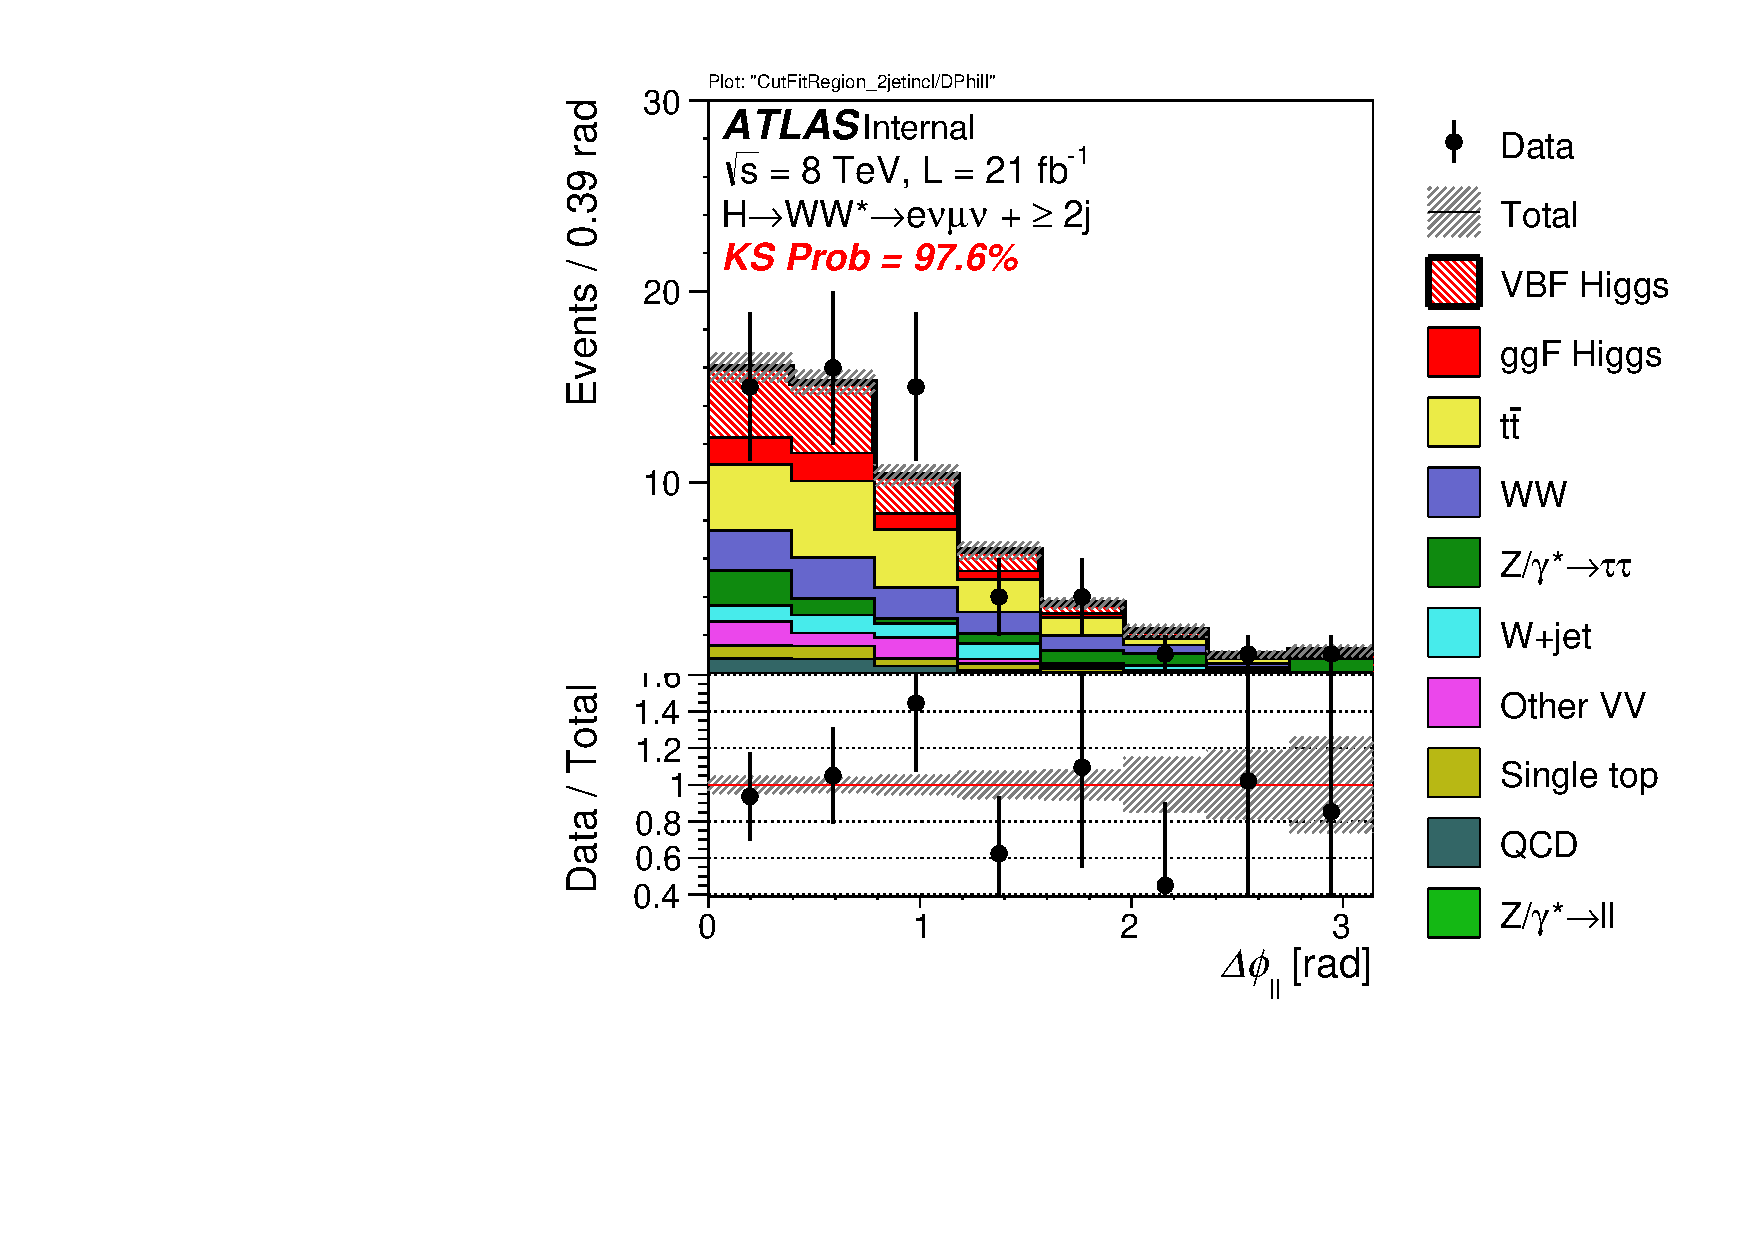
\includegraphics[width=0.4\textwidth]{fig/analysis/BDTinputVarsInSR/DF_SR_FitRegion_DPhill_mh125_lin.pdf}
   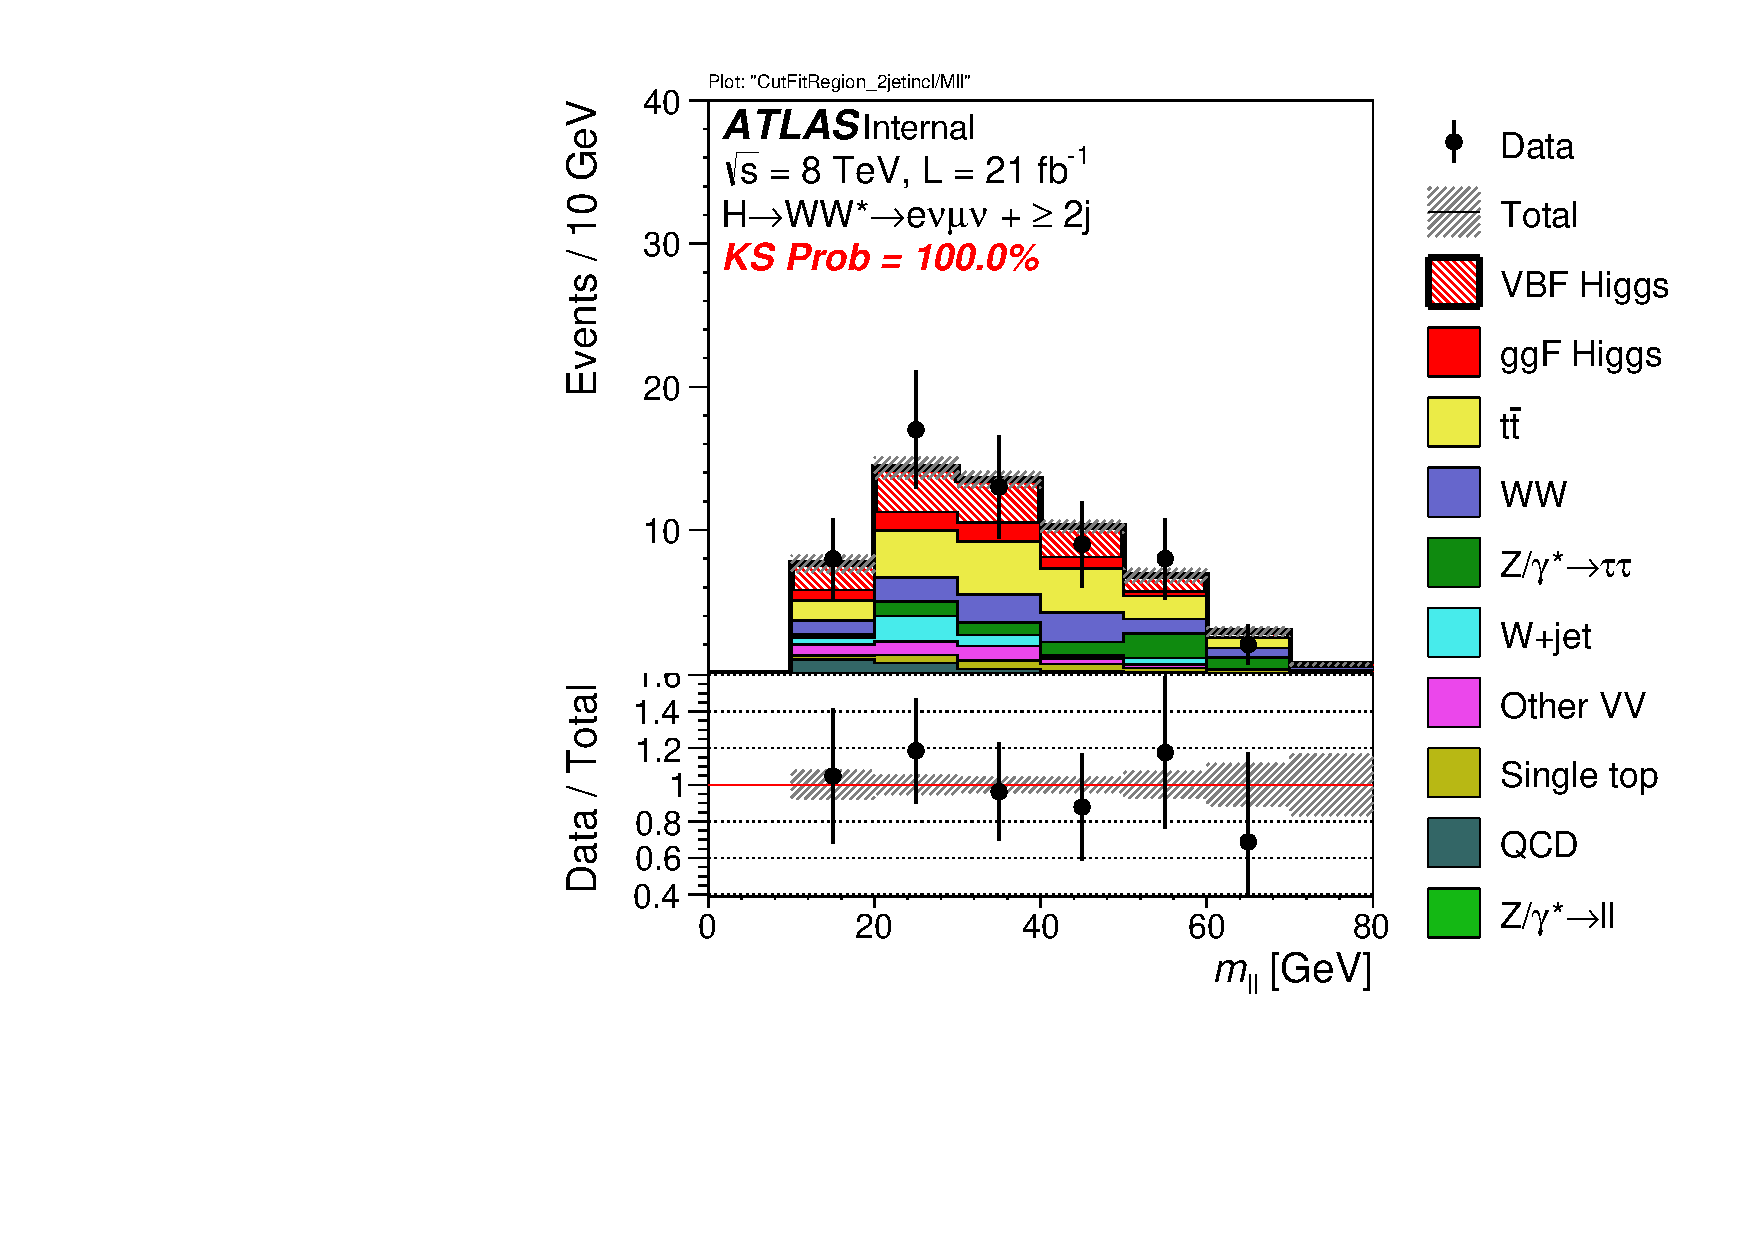
\includegraphics[width=0.4\textwidth]{fig/analysis/BDTinputVarsInSR/DF_SR_FitRegion_Mll_mh125_lin.pdf}
   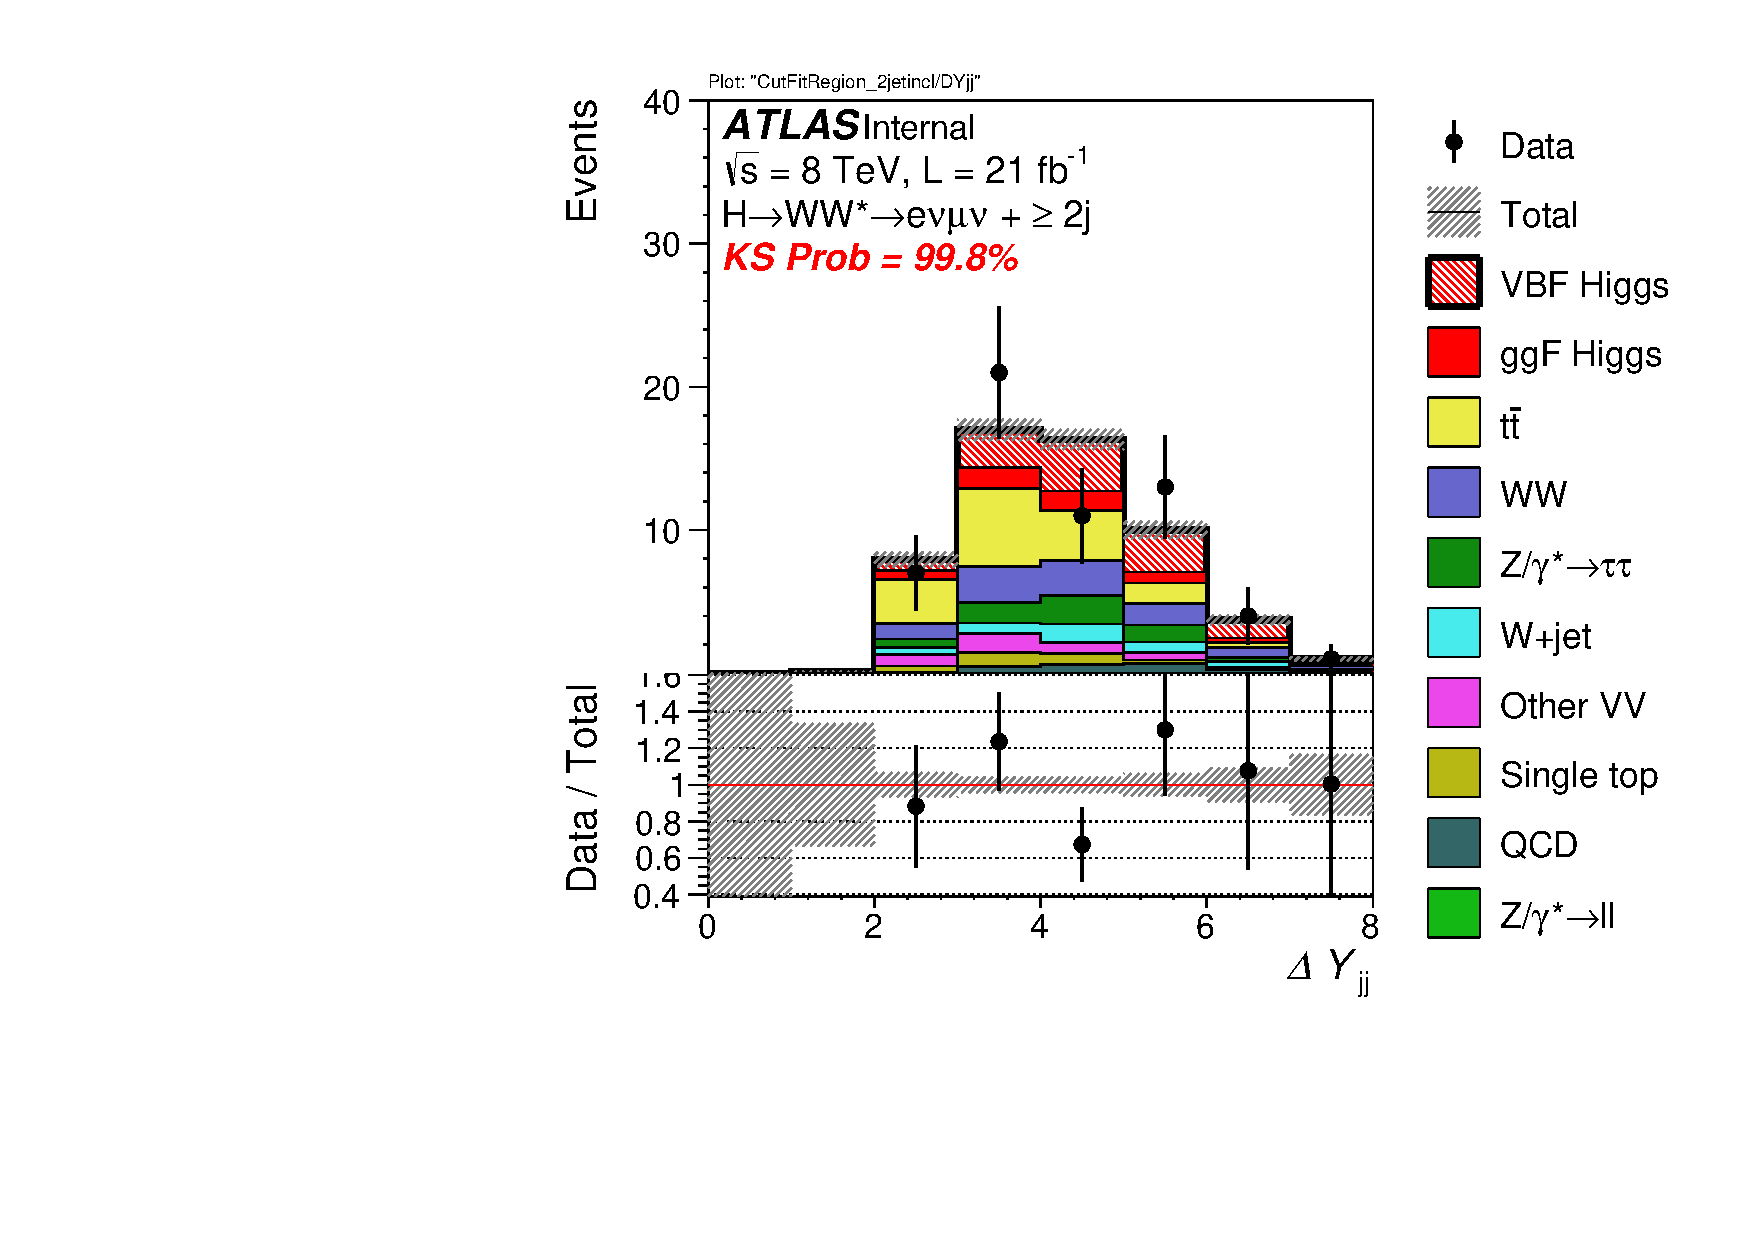
\includegraphics[width=0.4\textwidth]{fig/analysis/BDTinputVarsInSR/DF_SR_FitRegion_DYjj_mh125_lin.pdf}
   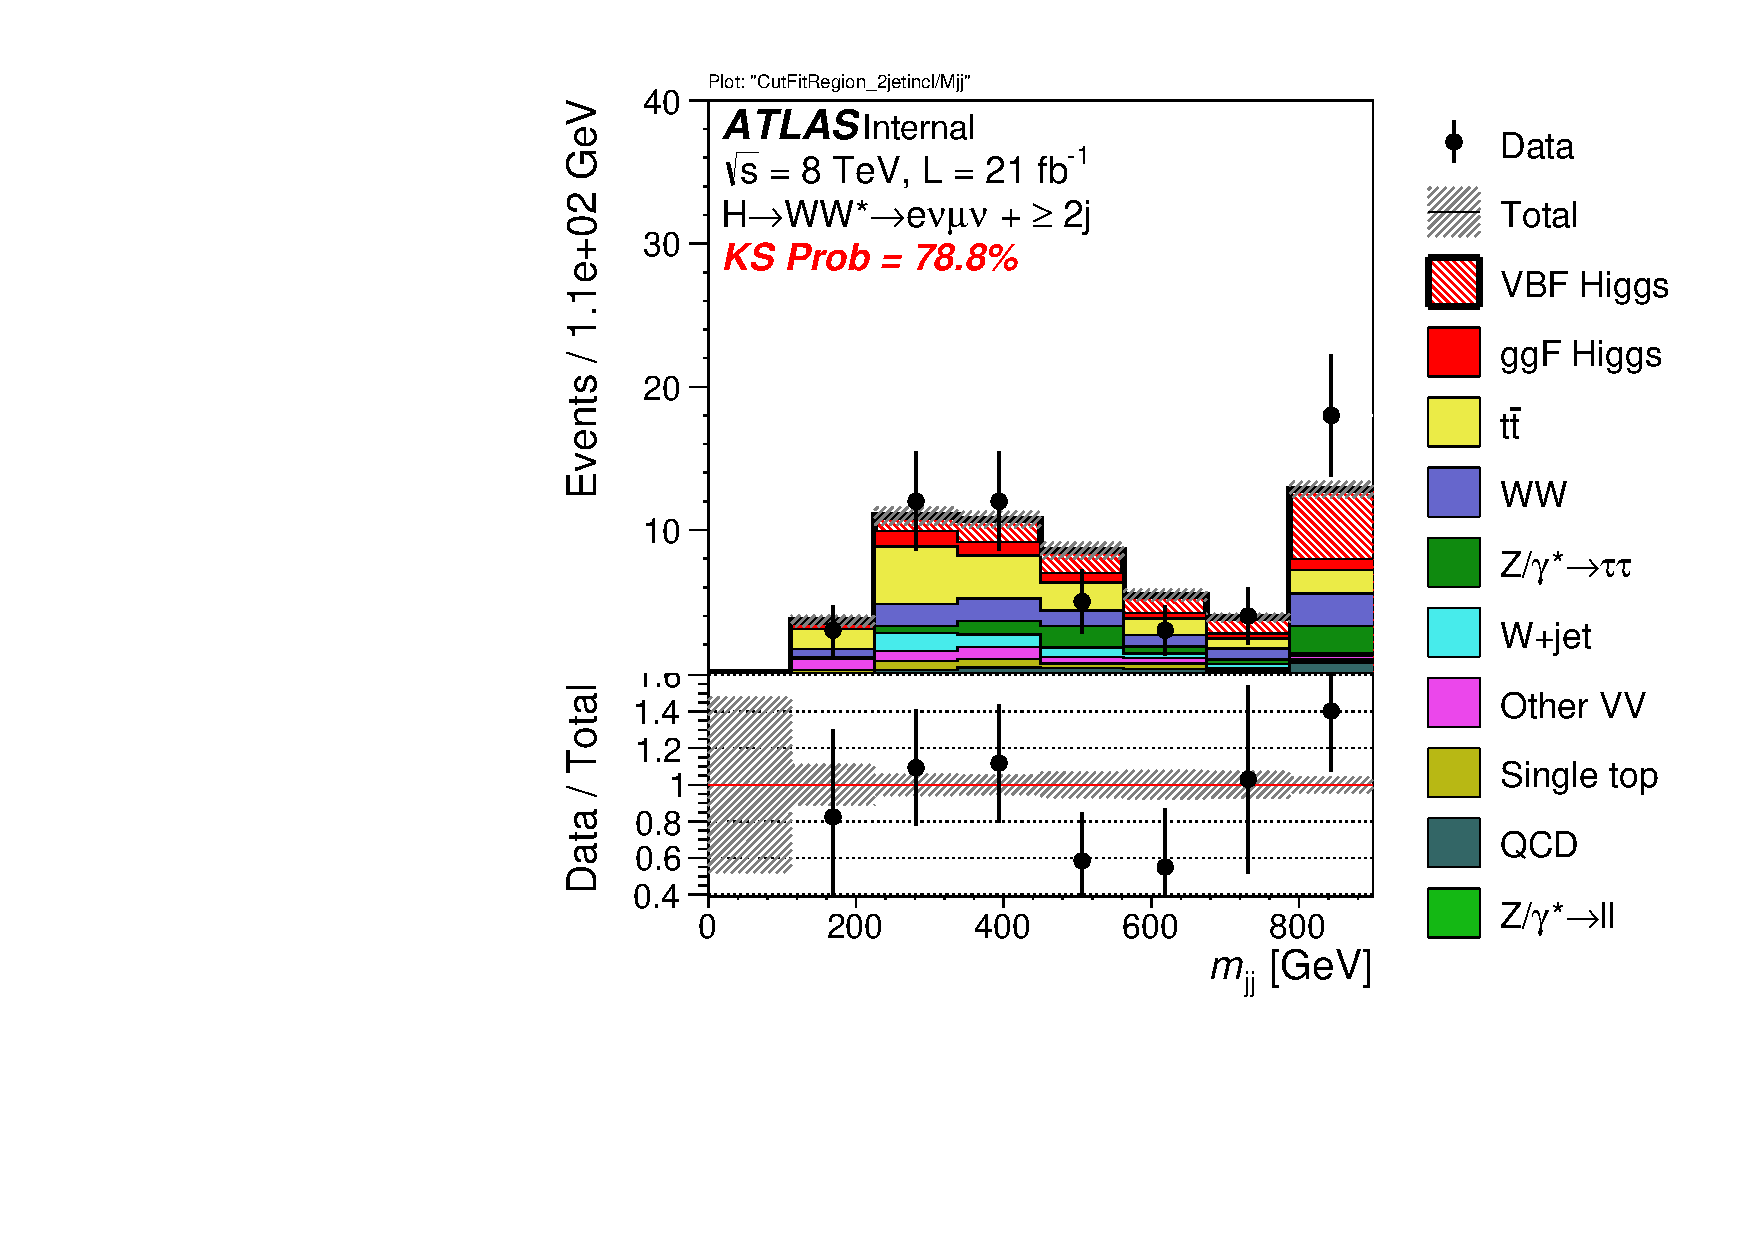
\includegraphics[width=0.4\textwidth]{fig/analysis/BDTinputVarsInSR/DF_SR_FitRegion_Mjj_mh125_lin.pdf}
   \includegraphics[width=0.4\textwidth]{fig/analysis/BDTinputVarsInSR/DF_SR_FitRegion_Pttot_tr_mh125_lin.pdf}
   \includegraphics[width=0.4\textwidth]{fig/analysis/BDTinputVarsInSR/DF_SR_FitRegion_MT_tr_mh125_lin.pdf}
   \includegraphics[width=0.4\textwidth]{fig/analysis/BDTinputVarsInSR/DF_SR_FitRegion_SumOFMvaMLepxJety_mh125_lin.pdf}
   \includegraphics[width=0.4\textwidth]{fig/analysis/BDTinputVarsInSR/DF_SR_FitRegion_contOLV_mh125_lin.pdf}
   \caption{Distributions
   of the eight BDT inputs \dphill, \mll, \dyjj, \mjj, \pTtot, \mT, \SumMlj, and
   \lepEtaCent
   in the \emme channel in the BDT signal region ($\textrm{BDT} > -0.48$).}
  \label{chap:analysis:fig:bdt_inputs_sr_df}
\end{figure}

\begin{figure}[p!]
  \centering
   \includegraphics[width=0.4\textwidth]{fig/analysis/BDTinputVarsInSR/SF_SR_FitRegion_DPhill_mh125_lin.pdf}
   \includegraphics[width=0.4\textwidth]{fig/analysis/BDTinputVarsInSR/SF_SR_FitRegion_Mll_mh125_lin.pdf}
   \includegraphics[width=0.4\textwidth]{fig/analysis/BDTinputVarsInSR/SF_SR_FitRegion_DYjj_mh125_lin.pdf}
   \includegraphics[width=0.4\textwidth]{fig/analysis/BDTinputVarsInSR/SF_SR_FitRegion_Mjj_mh125_lin.pdf}
   \includegraphics[width=0.4\textwidth]{fig/analysis/BDTinputVarsInSR/SF_SR_FitRegion_Pttot_tr_mh125_lin.pdf}
   \includegraphics[width=0.4\textwidth]{fig/analysis/BDTinputVarsInSR/SF_SR_FitRegion_MT_tr_mh125_lin.pdf}
   \includegraphics[width=0.4\textwidth]{fig/analysis/BDTinputVarsInSR/SF_SR_FitRegion_SumOFMvaMLepxJety_mh125_lin.pdf}
   \includegraphics[width=0.4\textwidth]{fig/analysis/BDTinputVarsInSR/SF_SR_FitRegion_contOLV_mh125_lin.pdf}
   \caption{Distributions
   of \dphill, \mll, \dyjj, \mjj, \pTtot, \mT, \SumMlj, and
   \lepEtaCent
   in the \eemm channel in the BDT signal region ($\textrm{BDT} > -0.48$).}
  \label{chap:analysis:fig:bdt_inputs_sr_sf}
\end{figure}




\section{\sqrts$=7$ TeV Analysis}
\label{chap:analysis:sec:reanalysis}

\section{\hwwlnln Analysis in Other Jet Bins}
\label{chap:analysis:sec:zero_one_jet}




